\documentclass{article}
\usepackage{graphicx,wrapfig,lipsum} % Required for the inclusion of images
%\usepackage{natbib} %bibliography style
%\usepackage[english]{babel}
\usepackage{amsmath} % Required for some math elements 
\usepackage{caption}
\usepackage{listings}
\usepackage{setspace}
\usepackage{verbatim}
\usepackage[margin=1in]{geometry}
\usepackage[percent]{overpic}
\usepackage{animate}
\usepackage{caption}
\usepackage{subcaption}
\usepackage{hyperref}
\usepackage{media9}
 \usepackage{movie15}
\usepackage[T1]{fontenc} % optional
%\renewcommand{\labelenumi}{\alph{enumi}.}
\usepackage{color} %red, green, blue, yellow, cyan, magenta, black, white
\usepackage[export]{adjustbox}
\usepackage[margin=1in]{geometry}


\definecolor{mygreen}{RGB}{28,172,0} % color values Red, Green, Blue
\definecolor{mylilas}{RGB}{170,55,241}
\definecolor{vblue}{RGB}{49,49,255}

\lstset{language=matlab,%
    basicstyle=\footnotesize\ttfamily,breaklines=true,
    breaklines=true,%
    morekeywords={matlab2tikz},
    keywordstyle=\color{vblue},%
    morekeywords=[2]{1}, keywordstyle=[2]{\color{black}},
    identifierstyle=\color{black},%
    stringstyle=\color{mylilas},
    commentstyle=\color{mygreen},%
    showstringspaces=false,%without this there will be a symbol in the places where there is a space
    numbers=left,%
    numberstyle={\tiny \color{black}},% size of the numbers
    numbersep=9pt, % this defines how far the numbers are from the text
    emph=[1]{for,end,break},emphstyle=[1]\color{red}, %some words to emphasise
    %emph=
    }
%bibliography style 
\usepackage[style=ieee]{biblatex}
\addbibresource{project_def.bib}
\DeclareLanguageMapping{english}{ieee}
\begin{document}
%%TITLE PAGE
% Logo
\begin{figure}
\vspace{-2cm}
\hspace{-2cm}

\includegraphics[width=\linewidth]{ubc_logo_ENG.eps}
\end{figure}

\linespread{1.3}\selectfont

% Title
\title{\bfseries{Capstone Final Design Report:\\Development and Optimisation of an Industry 4.0 Framework for Composites Manufacturing} \vspace{1cm}} 

\pagenumbering{roman}
\author{
\LARGE Faculty Advisor: Dr. Abbas Milani \\
\LARGE Clients: Bryn Crawford \& Reza Sourki \vspace{3cm}\\ 
\Large Group 34 Authors: \\ 
\Large Graeme Paul\\ 
\Large Daara Abbassi-Mohadjel\\
\Large Darryl Lam\\
\Large Louie Federico\\
\Large Connor Gaudreau\\ 
}

% Date for the report
\date{\vspace{5cm} \Large Date of Submission: April 12, 2020} 
%%END TITLE PAGE

\maketitle
\thispagestyle{empty}
\newpage

\pagenumbering{roman}
\tableofcontents
\clearpage

\begingroup
\linespread{1.3}\selectfont
\listoffigures
\addcontentsline{toc}{section}{List of Figures}
\endgroup
\clearpage

\setlength{\parskip}{1em}
\setlength{\parindent}{0pt}

\linespread{1.3}\selectfont

%\addcontentsline{toc}{section}{List of Figures}

\addcontentsline{toc}{section}{Executive Summary}
\section*{Executive Summary}
At UBC Okanagan’s School of Engineering, fourth year engineering students are required to complete the two semester Capstone design project. Over these two semesters, students of all engineering disciplines work in teams to solve a specific design problem for a client. For this  project, our client was the UBCO Composites Laboratory with the project supervisor Bryn Crawford. This report’s purpose is to detail the project’s final design and the results achieved over the 2019/2020 semesters.  The final report contains the project's needs and constraints, problem specification, design process, solution generation, final design details, and the final design’s evaluation. The project’s fundamental design problem is finding a solution for improving the manufacturing process of composite materials by specifically optimizing the curing cycle of composite materials. The goal was to replace the controller for the composite curing oven which is a standard PID controller with a smart solution implementing Industry 4.0 concepts. Industry 4.0 is the new paradigm digitizing and automating the industrial sector by using digitally connected sensors, machine learning, and real-time data usage. To complete this task, the needs were catalogued. The main needs were established to be finding the soak/cure time through the usage of machine learning and implementing a data collection unit to attain data. Based on this need of finding cure time, a solution was generated and selected by doing an extensive literature review, analysing the key findings, and creating a feasible solution. \\\\
Two machine learning implementations were selected for the preliminary design. The first was random forest which uses decision trees to make predictions on data. The second was long short term memory (LSTM) which is based on a recurrent neural network and is a more traditional neural network machine learning algorithm. To gather data, a Raspberry Pi and ADC were used together to read NTC thermistors inside of the heating chamber. A modified part which allowed for a thermistor to be inserted provided truth data which was used to train the neural network. Air temperature data inside the heat chamber over a cure cycle was also collected which became the input data to be used to make a prediction with the machine learning algorithms. In addition to real data, simulations were used to develop additional data to help iterate and tune our designs. After turning the machine learning algorithms and setting the necessary parameters, a prediction capability with a percent error of under 4\% for the entire run was found. Due to the COVID-19 virus suspending laboratory times, we encountered further constraints that limited testing and the amount of data that could be collected in the lab. Code was then created to estimate the soak time, make future predictions on data, and return control decisions based on machine learning predictions. It was concluded that our implementation provided a good estimate  of the internal temperature of the part . Finally, our recommendations for future topics which could be researched to improve or expand the project include additional validation and testing, implementation with a cloud service for data storage, data assimilation, transfer learning, and improved simulations. 

\clearpage

\pagenumbering{arabic}
\section{Introduction} \label{introduction}
The UBCO Composites and Optimization Lab is interested in modernizing the production and fabrication of fibrous and polymeric composites, known as composites manufacturing. The modernization of these processes using the technologies developed over the past two decades is encompassed by the manufacturing paradigm of Industry 4.0. By focusing on the specific process of composite curing, a framework for applying Industry 4.0 principles to composite manufacturing processes can be developed. \\\\
Composite curing is the process of heating a composite material until it reaches a specific internal temperature, in which it undergoes a chemical strengthening process. This temperature will be reached at a specific time, the soak time, which is determined, but not easily calculable, by the initial conditions and physical parameters of the material. This entails that an object heated for its soak time will be cured. For a manufacturing process, the materials are heated in a curing oven, which on a large scale can be expensive to run. In a lab environment, where the soak time of a given material may not be known, curing ovens are left to run much longer than what could reasonably be deemed necessary to compensate for this uncertainty. To minimize the expense, and thus the time the oven is left running for, a new method to determine the soak time for a given material needs to be found. \\\\
Industry 4.0 is a modern paradigm in manufacturing processes whose principles include inter-connectivity, information transparency and decentralized decisions. In practice this amounts to using internet-connected technology to make data-driven decisions for the manufacturing process. With regards to composite manufacturing, the technological framework to accomplish this would include digitally-connected sensors, a centralized database, machine learning, and microcontrollers. For the specific process of composite curing, the sensors would detect temperature and relay this information back to the processing unit, which could then control the curing oven accordingly. By establishing a solution under Industry 4.0 principles, a transferable workflow can be established forming a basis for future research. \\\\
The objective of our project is then to apply the principles of Industry 4.0 to optimize the composite manufacturing process of composite curing. This report will detail the problem formulation, design process, the end product and an evaluation of the overall success of the project. \\\\

\clearpage

\section{Problem Specification} \label{Problem_Specification}
The main objective of our project was creating an Industry 4.0 framework using a machine learning model to optimize the curing process by accurately estimating the soak time required. Specifically for our case, as a proof of concept we acquired an aluminum cylinder with a radius of 3cm and length of 5cm. The purpose of this proof of concept was to address the problems with the current solution in the UBC Okanagan Composites lab. It was expected that the new framework would implement Industry 4.0 principles integrating data acquisition devices with machine learning. Our clients also expressed a desire for the framework to have the sensor data and the machine learning model uploaded online to the IBM Cloud service. This desire was however dependent on time and costs because the IBM Cloud adds costs based on data usage. Therefore it was clearly stated that the amount of data should be limited as much as possible. However, building a robust machine learning model often requires large amounts of data for training and testing. For addressing the issue, we did not specify a maximum numerical value for the amount of data collected, instead we looked to reduce the amount of data used for training and testing the model until its performance suffered significantly. Using this strategy would be key to producing a framework to satisfy the problem.\\\\
The temperature range to be used for curing parts was specified by the client early in the project. The allowable range was between 25$^\circ$C and 80$^\circ$C for curing parts. Therefore any material placed inside the heat chamber had to be capable of withstanding temperatures of at least 80$^\circ$C. However, our clients did have aspirations for using the final product to test composites at temperatures over 200$^\circ$C. Therefore the specification for our final solution included handling temperatures up to 250$^\circ$C which was the maximum temperature the thermistors could withstand. 
As the project budget was limited to \$300, it was necessary to minimize the cost of hardware devices used for our final design. To stay within budget, we limited our costs on hardware down to devices which included a 16 bit ADC for data acquisition, and a Raspberry Pi for storing the data from the ADC and extracting it for analysis. Ultimately by limiting the costs of hardware devices, we were able to stay within the \$300 budget.
\clearpage

\section{Needs and Constraints Identification} \label{Needs}
\subsection{Stakeholders}
The official partner involved in this project is The Composites Research Network (CRN) Okanagan node. The CRN is a group of several Canadian universities and industry partners involved in composites manufacturing. The purpose of the CRN is having academic institutions and industry leaders collaborate to find solutions to problems facing the composites manufacturing industry \cite{crn}. The resulting intellectual property produced from this project could impact the members of the CRN outside of the Okanagan node, so they’re considered external stakeholders even though they were not consulted during this project.

The main stakeholders for this project are Project Supervisor Bryn Crawford, Facility Supervisor Dr. Abbas Milani, and Ph.D. student Reza Sourki at UBC Okanagan campus. These main stakeholders work at UBCO’s Composites and Optimization Laboratory doing research and development on polymeric composite materials. The Project Supervisor Bryn Crawford and Reza Sourki were met with throughout both semesters. Meetings consisted mostly of conceptualizing the problem and understanding their expectations in the first semester. Once the problem was defined, meetings transitioned towards providing updates and progress reports.

The main internal stakeholders at the UBC Okanagan Composites and Optimization Laboratory were impacted positively by the results of this project. Their needs for minimizing soak time and accurately predicting the curing cycle of a composite material were met to an acceptable level. The intellectual property created can also impact other laboratories in the CRN doing composites research and development. There could be benefits for these labs if our framework is adjusted to work for predicting the curing cycle on more complex composite materials.

\subsection{Needs}
Through early discussions with the stakeholders and group meetings, the needs for the project were established. It was found that the main need was to accurately predict a composite's internal temperature and minimize the soak time of the curing cycle. Also made clear by the stakeholders was the need to implement an Industry 4.0 framework creating an innovative and robust final design.\\\\
%The main purpose of this project was to satisfy the needs not being met by the solution in UBC Okanagan’s composite and optimization lab. The main problem with the current solution was the soak time could not be accurately estimated. This led to more power being consumed than necessary in the heat chamber and the possibility that composites are of poorer quality. We knew addressing the main needs was key to reducing the total amount of time for curing a composite material. Another important need to satisfy was building a framework capable of estimating soak times across a wide range of composite materials. This framework also needed to be capable of estimating soak times for varying part geometries, materials, and thermal properties. \\\\
The stakeholders expressed an additional need for implementing an Industry 4.0 framework, combining sensors with machine learning algorithms for estimating soak times. It was determined that using machine learning algorithms would provide a more robust solution.  This meant the framework had to include a way for users to easily store and manipulate data. Finally, the idea of designing a process for uploading data to the IBM Cloud service was expressed if it was feasible. This would give the stakeholders a way of accessing data across multiple devices and provide a platform for doing data calculations. Due to the cost of storing extensive amounts of data, it was defined that our implementation should try to limit the amount of data as to minimize the burden of costs on the lab. It was determined that meeting these needs defined by the project stakeholders would satisfy the requirement of producing an Industry 4.0 framework for this project.\\\\
Accurately finding a given part’s internal temperature over time for the purpose of reducing soak time was considered the most important need for this project. The solution had to satisfy the main need using Industry 4.0 principles including data collection, data streaming, machine learning, and cloud services. Lastly, the overall design framework required detailed documentation so it could be easily replicated over a range of composites.

\subsection{Scope and Constraints}%Many constraints were identified during the definition stage of this project. The main purpose for this project was to develop an Industry 4.0 framework for optimizing the composite curing process. The scope for this project was to build this framework using a machine learning algorithm that estimates the soak time of a metal part with simple geometry. 
Many constraints were identified during the definition stage of this project. The scope of the primary deliverable was building a framework for obtaining internal part temperature using a machine learning algorithm for simple metal cylinders and using this data to estimate the soak time. Studying objects with different materials, sizes, and shapes were considered within the project’s scope if the primary deliverable was completed before the project’s deadline. Metal cylinders were proposed by the stakeholders as the limit of our scope for testing and implementing our Industry 4.0 framework because the heat transfer characteristics are easily known whereas for composite parts the characteristics are not always available. So estimating soak times on composites with epoxy exhibit exothermic properties was considered outside the scope of this project in order to simplify the process for developing a framework.
\\\\
With a budget of \$300, the primary cost constraints were first identified for the project. These included temperature-based sensors, data collection devices like Arduinos and Raspberry Pi, and costs of acquiring metal parts. NTC 100k Thermocouples were implemented for sensing air temperature and part temperature in the heat chamber. Also a 16 bit analog-to-digital converter (ADC) microcontroller and Raspberry Pi were used for creating the data acquisition system for storing and streaming real-time data from the curing cycles. It was planned to store data on the IBM Cloud computing service keeping in mind the volume of data would lead to higher monthly costs for storing this data thus data must be minimized.% It was found that the amount of data collected depended on the number of thermocouples, and the amount of tests performed. Therefore it was an objective to minimize the amount of heat chamber tests performed and find the minimum number of thermocouples without jeopardizing the accuracy of the results. Also the configuration of the thermocouples inside the heat chamber had to be considered for ensuring accurate temperature measurements.
\\\\ 
It was found that the accuracy of the thermocouples was critical because the data collected would be used for training and testing our machine learning algorithms to estimate a part’s internal temperature and soak time required. Therefore constraints on the thermocouples and all hardware devices had to be considered such as the latency and signal-to-noise ratio. To satisfy these constraints, it was important to ensure that the measurements obtained by the hardware devices in this project were consistent and repeatable under specific testing conditions.
\clearpage
The amount of tests performed was also a recognized constraint as it placed restrictions on the volume of data collected and time availability. An objective was to determine the amount of tests necessary for obtaining a large enough data set to meet our expectations. It was found that the time consumed for a single test depended on the target temperature, thermal properties, and the size of the metal cylinder.  Due to these constraints we selected an aluminum cylinder with a 3cm radius and cured it at lower temperatures than typically used for composite curing to have more test runs and a larger data set. Another strategy for meeting these time constraints related to test runs was implementing MATLAB heat simulations to generate more data sets for training our machine learning algorithms and testing them.\\\\
There were some risks identified during this project with regards to health and safety. There were potential dangers working with the heat chamber and infrared lamp because of the high temperatures involved. It was necessary to practice the safety precautions laid out by our clients when using the lab equipment. There was minimal technical risk of losing data due to the use of cloud storage and revision control. Finally there were no significant environmental or societal impacts to be considered within the project's scope.

\clearpage

\section{Solution Generation and Selection} \label{Solution_Generation}
\subsection{Previous Solutions by Stakeholders}
To define the problem with the current solution, an assessment of the client’s current solution was done. The lab was using a heat chamber with an infrared (IR) lamp as the heating source for curing composites. Inside the heat chamber, three thermocouples are used to measure the air temperature. Due to variability in temperature inside the chamber and variability between the sensors themselves, an average of all the thermistors are used as the temperature which the Ardiuno acts on. This average value gives an accurate enough reading of the air temperature recorded over the entire curing run. The chamber uses a PID controller which controls the IR lamp by sending a PWM signal to a MOSFET. The heat chamber’s temperature rises a few degrees per minute until the desired curing temperature is reached. As specified earlier, the heat transfer characteristics of a composite part are not easily determined, and therefore the soak time cannot be analytically determined. The method currently used is to hold a part at the target temperature for a period of time determined heuristically. This time is long to ensure the part temperature reaches the threshold and is cured completely. This is where the current solution needed improvement because the minimum soak time required for the part to reach equilibrium temperature was being exceeded. Because of this, the heat chamber was being used longer than necessary which led to wasted time and power.

\subsection{Industry Solutions}
When initially formulating solutions to the problem, a literature review was done to assess current industry solutions for accurately predicting part temperature and estimating soak time. This section reviews current industry solutions for optimizing composite curing and evaluates their potential application to this project. \\\\
It was found the key parameters involved in the cure cycle are the heat transfer characteristics, material properties, heat convection through the material, and surrounding air temperature. In the composites manufacturing industry, using control strategies and numerical simulations is a technique for developing an optimal cure cycle. The numerical simulations involve adjusting parameters previously mentioned to build prediction models for improving the degree of cure and minimizing the total time of cure. By defining boundary conditions inside the heating chamber, finding an energy equation combined with a kinetic model, and using finite element software, the degree of cure and temperature across a composite can be simulated \cite{curesim}.  Here the numerical simulations showed the degree of cure and temperature at various points on the composite with different thicknesses. The paper however did not have experimental data of an actual cure cycle to compare with the simulation results. This process can be validated as seen in \cite{polylam} which used similar numerical simulations and had results showing accurate estimates of part temperature and better degree of cure at various points on the composite. The solutions proposed in these studies struggle to address the problem of producing a non-uniform temperature distribution across composite materials. This causes some spots on the composite to be burnt and others processed below the desired temperature. Also, the models still cannot always accurately predict the soak time.\\\\
Another possible solution was a self-tuning method used for finding the optimal curing parameters using a programmable microcontroller to create a self-tuning algorithm \cite{selftune}. First, the oven parameters were used to create an electrical model and then derive a differential equation which could be used for finding an optimal cure cycle. A PID controller was implemented to adjust the oven temperature based on the differential equation and electrical model. Finally, simulation results were compared with experimental results to prove the self-tuning method’s accuracy. The results of this study reveal similar problems found with our clients curing process, such as the inability to fully predict when the part is within the desired curing temperature. The solution also does not provide the level of innovation we hoped to achieve in this project.

\subsection{Machine Learning Applications in Composite Curing}
For this project it was desirable to implement an Industry 4.0 design as a solution, and specifically an Artificial Neural Network (ANN). The motivation behind this decision was supported by evidence from literature on applying an ANN to composites curing. It was also found that the problems associated with the other current solutions discussed earlier can be mitigated using an ANN, from sources such as ’Prediction and optimization of cure cycle of thick fiber-reinforced composite parts using dynamic artificial neural networks’ \cite{ann}. This study implemented a neural network with the purpose of optimizing cure cycles using the surrounding air temperature and the characteristics of the composite. This goal is achieved by first building a finite element model (FEM) on the composite part. The FEM provided sample data of the variables time, autoclave temperature, and composite part temperature at specific points. Then this data was used for both training and testing two different neural networks. One network was used to model the output and control of the composite’s temperature and the other for the composite’s degree of cure. Doing this allowed them to see relationships between a part’s temperature and the degree of cure at various points on the part. The study then looked at several different training algorithms and found Bayesian Regularization had the strongest prediction ability. Also, it was found that making changes to the ANN architecture like changing the number of neurons had no significant changes to the predicted output. Overall, the ANN applied in showed results that reduced soak time and accurately monitored a given part’s internal temperature.\\\\
Then in ‘Optimization of the Temperature-Time Curve for the Curing Process of Thermoset Matrix Composites’ \cite{rnn} it showed a recurrent neural network (RNN) which is a specific type of ANN. This was applied towards optimizing cure cycles and producing a uniform cure on fiber-reinforced thermoset matrix composites. The RNN used two hidden layers between the input and output layers which allowed for increased prediction ability without adding significant amounts of time to train the network. This structure also allowed the number of neurons to be decreased because the additional hidden layer’s outputs are fed back into the network. As before, there were two RNN’s used, one for predicting the composite’s temperature and one for the degree of cure. The results produced by the RNN’s showed the optimal curing times for a composite which achieved a uniform degree of cure across the material. These results are relevant to our project because having a solution that achieves a uniform cure across a material is important to the client. These papers use epoxy parts with complex properties which are outside the scope of this project. However, the concept of training an RNN with data generated from a FEM is still useful for this project.

\subsection{Project Workflow}
To facilitate the solution generation process, a project workflow was developed. While this project was focused on designing for a specific task, the overall goal was to develop a generic workflow for applying Industry 4.0 principles to composite manufacturing processes. The workflow was generated at the start of the concept generation part of our design, allowing other solutions to fit in with each of these points. The abstracted workflow for the project was developed as follows:
\begin{enumerate}
\item Identify all input and output parameters of process
\item Use Industry 4.0 technology to automate data collection of input and output parameters
\item Process input and output data into supervised learning data sets, in which each set of inputs is mapped to one output
\item Determine models most applicable to current problem and eliminate others 
\item Design machine learning models to take input parameters and produce output parameters
\item Train ML models using collected supervised learning data set
\item Determine models that are working well with data set and eliminate others
\item Refine model parameters to enhance predictive accuracy
\item Validate model with test cases, including fringe examples
\item Integrate machine learning module into data collection network
\end{enumerate}
\subsection{Machine Learning Model Selection}
Machine learning algorithms can be categorized into four main types: supervised learning, unsupervised learning, semi-supervised learning, and reinforcement learning. In supervised learning, the algorithm takes training data and generates a function made up of biases and weights that relates the input features to the output labels of the data sample. The goal of supervised learning is to train the algorithm on known data in order to later predict on unknown data. In unsupervised learning, the algorithm does not have access to the output labels. In this case, the goal of the algorithm is to model the structure or distribution of the training data in order to later predict on unknown data. Semi-supervised learning can be considered part supervised learning and part unsupervised learning. In this case, the data contains some output labels, but output labels are not present in all of the data. In reinforcement learning, like unsupervised learning there are no output labels to train the algorithm. Rather than trying to model the structure or distribution of the data, reinforcement learning uses an agent that learns through experience and tries to maximize reward which is defined by a reward function.\\\\

Additionally in machine learning, there are two main categories of tasks: regression and classification. In regression tasks, the output label being predicted is numerical while in classification tasks, the output label is a category. In our case, the problem of finding the internal temperature of an object is a regression task.\\\\
Supervised learning was selected as the most suitable machine learning domain for our use case, as it is difficult to determine the optimal machine learning algorithm for an application without testing and comparing the results. Selection of models was also aided by the structure of inputs and outputs. Machine learning models that work well with time series data and output a real number should be prioritized. %In this manner, broad classes of machine learning were able to removed, %such as regressions due to their inputs, and classification models due to their output. \\\\

\subsubsection{Machine Learning Development Platform Selection} \label{ML_platform}
As part of our concept generation we had to decide how to implement the machine learning models described. There are many possible languages and packages which can implement these algorithms. Two languages which our group was both familiar with and had well-documented libraries were Python and MATLAB. Python was chosen due to the packages available, flexibility, experience of our group members, and preference.
\paragraph{Keras and Tensorflow} \, \\
Tensorflow is an open-source library for numerical computation and large-scale machine learning. Keras is used as a high-level neural network API for Tensorflow. Keras was chosen for this project due to its accessibility in implementing machine learning algorithms using Tensorflow. With Keras, we were able to implement the various RNN model types, such as LSTM and GRU, using Python. Using these tools, we were able to train and run the RNNs from the data gathered to accomplish our project needs.

\paragraph{Scikit-Learn}\, \\
Scikit-Learn is a machine learning library for Python. Scikit-Learn was used for this project due to its simplicity in implementing the Random Forests machine learning algorithm. It also enabled us to remain consistent with using Python for all our implementations of the machine learning methods.  
\subsection{Simulation Tools}
MATLAB was chosen because of its built-in toolboxes and functions like the Partial Differential Equation (PDE) Toolbox™. This toolbox can be used for solving partial differential equations and FEM heat transfer problems \cite{matlab}. The PDE toolbox allows users to create a thermal model which holds the geometry, boundary temperatures, initial conditions, and material properties of the thermal system and simulate the transient response. Furthermore, the entirety of the group was familiar with MATLAB. This provided a basis to get into the complex field of heat simulation while focusing on more pertinent problems.
\clearpage

\section{Design Process} \label{Design}
As the project was both modular and largely virtual, large scale prototypes were not developed. The two large components of the project, the data acquisition unit and the machine learning unit, were developed concurrently with their integration being overseen as the final step. As the data acquisition unit was simple in comparison there was no need found for a preliminary design. For the software components, the design was continually iterated upon and tweaked until desired results were obtained with all iteration tracked using the revision control software Git. Therefore the preliminary software implementation in our design slowly morphed into the final design through iterating upon it. 

\subsection{Design Process of Data Acquisition}
The basic concept for data acquisition was to measure the air temperature of the curing oven as well as the internal temperature of an aluminum cylinder. The preexisting curing oven setup was used, being controlled by a PID controller being fed air temperature data using the average of four 100k NTC thermistors. \\\\
For the first design, air and internal temperature measurements were taken using five 100k NTC thermistors to ensure consistency with the original setup and to determine an accurate temperature profile for the immediate vicinity of the cylinder. The temperature data was read and logged by a Texas Instruments TM4C123G microcontroller, which was chosen due to its affordability. The cylinder was suspended by a wire cage, to maximize the thermal absorption of the cylinder. \\\\
While this setup produced data relatively consistent with what was expected, a number of issues were identified.
The biggest issue was the variance in temperature readings between the thermistors. A 3 degree difference between them was found by exposing the thermistors to a constant heat source. As the machine learning model requires accurate data to provide accurate predictions, this posed a serious issue. Possible issues were determined to be faulty connections, an incorrect circuit configuration, a wrong thermal model, and the ADC on the microcontroller. Different thermistors produced the same variance, which implied that the issue laid in the ADC of the microcontroller most likely due to a faulty board.\\\\
Another issue came from a characterization of the temperature profile in the curing oven. While the temperature on the horizontal plane was constant, there was a steep temperature gradient vertically, which entailed that the inconsistency of the wire suspension setup would make it difficult to generate reproducible data. On the other hand, the constant temperature on the horizontal plane eliminated the need for many thermistors, as only 3, for the top, middle, and bottom of the object would be necessary to determine the air temperature. 
For the final design, a Raspberry Pi 4 microcontroller was used to read and log thermistor data, as its readings were found to be consistent when exposed to constant heat. As the position of the cylinder in the chamber was found to be a significantly larger influence on temperature than the existence of other thermally conducting masses, a wooden base was used to support the cylinder rather than the wire suspension. Studs were cut into the top to isolate the cylinder. The specifics of the final design are shown in Design Details section \ref{Design_Details} of the report.
\subsection{Simulation for Data Generation}
Using machine learning algorithms to predict the soak time for a curing cycle could possibly require a large amount of data for training and testing. During the planning stages of this project, we determined that heat chamber testing may be insufficient for generating the required amount and different types of data. In addition, simulation of the process allows us to tweak and iterate on the design with different data and different amounts of data easily. Physical tests would add extra cost and time running the heat chamber, along with the difficulty of acquiring parts with different materials, various geometries and properties. \\\\
To acquire data more economically, we found that the best way to address this problem would be to implement finite element software to build a thermal model and simulate curing cycle data sets, a technique used in articles from the literature review \cite{rnn}. %MATLAB was chosen because of its built-in toolboxes and functions like the Partial Differential Equation (PDE) Toolbox™. This toolbox can be used for solving partial differential equations and FEM heat transfer problems \cite{matlab}. The PDE toolbox allows users to create a thermal model which holds the geometry, boundary temperatures, initial conditions, and material properties of the thermal system and simulate the transient response.
Using the PDE Toolbox, we were able to model our aluminum cylinder and the heat chamber conditions then simulate the transient response for the system. Generating simulated curing cycles in MATLAB produces useful data sets with similar features to real curing cycle data. These simulations are important because providing a neural network or machine learning algorithm with data sets accurately representing real data sets will increase the robustness. The resulting simulations can effectively train and test a neural network, reducing the time and money needed for experimental testing needed for generating data sets. Fundamentally the simulated data allowed us to quickly iterate and tweak the machine learning system and check its validity in predicting under different circumstances.  %Once the neural network is sufficiently trained with the simulation data, it can be used for predicting real time data sets. This is the full methodology behind this process of generating simulated data sets.

\subsection{Machine Learning Model Design Process}
Through research and experimentation, we narrowed down the algorithms we were interested in and selected two final algorithms to implement and compare. The two supervised learning techniques that we focused on were Random Forests and RNN specifically Long Short-term Memory networks (LSTM). To better understand the applicability to our problem, we continued researching these two algorithms and implemented them into our preliminary design. \\\\
The fundamental design of these models are accessed through library's and packages mentioned in the Solution Generation in section \ref{ML_platform}. Both Keras/Tensorflow and Sci-kit learn were used to implement the bulk of the learning networks which make up the machine learning algorithms. This left us with having to design the machine learning parameters, implement the surrounding code to access the packages and libraries, and then output the performance of the machine learning processes. In addition to this, there was also the task of applying code to make predictions, and show the capability as a control source for the data acquisition unit. To quickly prototype the algorithm on larger data sets, the simulated data was used. The simulated data allowed us to quickly asses the feasibility of the machine learning algorithm and quickly iterate on the design to improve it. As mentioned above, iterating on software was simple with the help of revision control software. Once real data was obtained, the machine learning algorithms proved to be well designed because of the previous work done to validate our designs on the simulated data. \\\\
\clearpage

\section{Final Design Details} \label{Design_Details}
The final design can be segmented into 2 stages: the data acquisition unit and the machine learning unit. Connecting these two parts of the project is the data refinement process. In a broad overview, the data generated by either the heating chamber or the MATLAB simulation were processed and input into the Random Forests and LSTM neural network. Each component of this is detailed below.

\subsection{Data Acquisition}
The data acquisition unit consists of the curing oven, the PID control system, the temperature sensors that provide the temperature data, and the microcontroller that reads and logs the data. The curing oven and PID control system remain unchanged from their initial setup. %Due to the premature closure of the lab, no photographs of the setup were taken, as all equipment was left in the lab.

\subsubsection{Curing Oven Configuration}
The curing oven configuration consisted of four 100k NTC thermistors for recording the external air temperature around a test object with an internal thermistor. The object used in the experiment was an aluminum cylinder of 3 cm radius, and 5 cm height. A hole was drilled into the cylinder with a depth of 2.5 cm in which we inserted a thermistor. The metal cylinder was held by a raised 10cm wooden platform with studded ends. This was to keep the cylinder isolated from other heat sinks. A mockup of the design is shown in Figure \ref{fig:heat_chamber_cad} with the heat source in red, the cylinder in white, and the thermistors connected to the black wires. 

\subsubsection{Temperature Sensor Configuration}
The three external thermistors were placed close to the surface of the cylinder. They were positioned above, below, and on the side of the cylinder. It was found that due to constant temperature on the horizontal plane, any extra thermistors would unnecessarily increase the amount of data. While three thermistors were used, due to the vertical temperature gradient of the heat chamber, the central side thermistor was weighted higher than the other two for determining the average external temperature as it was reflective of the mean temperature due to symmetry.
\newpage
\begin{figure}[!htb]
    \centering
    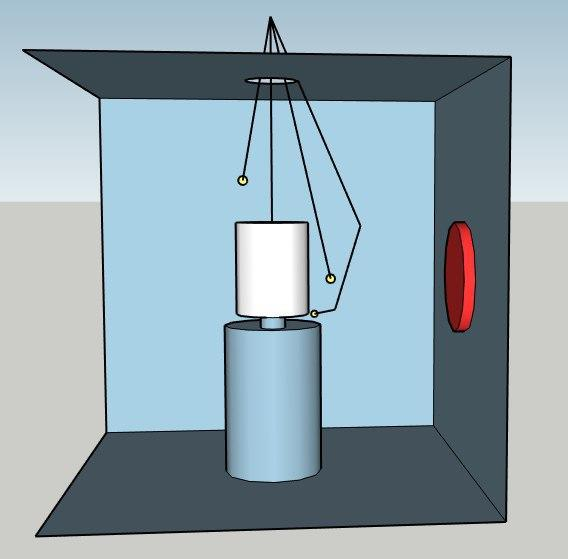
\includegraphics[width=0.4\linewidth, frame]{other/heat_chamber_cad.jpg}
    \caption{CAD Drawing of Heat Chamber Test Configuration}
    \label{fig:heat_chamber_cad}
\end{figure}
\subsubsection{Microcontroller Configuration}
The data we collected was collected on the TM4C123G. Our preliminary design initially developed consisted of thermistors connected to a Texas Instruments TM4C123G. To increase accuracy and computational power we changed our data acquisition unit to a Raspberry Pi 4 with an external ADC used to interface the thermistors to the Raspberry Pi. The ADC is connected to the midpoint of a voltage divider between the thermistor and a 100k $\Omega$ resistor. Steinhart-Hart equations shown below as Equation \ref{shheq1} \& \ref{shheq2} were used to covert the voltage reading to a temperature reading, using coefficients found from \cite{shheq} and the table \cite{ttable} containing resistance values for our thermistors along.    
\begin{equation} \label{shheq1}
    R_{thermistor} = \frac{100k \Omega}{ V_{dc} / (V_{dc} - V_{adc reading}) - 1.0}
\end{equation}
\begin{align*}
Where \\
c1 = 0.6764629190e-03 \\
c2 = 2.230798167e-04 \\
c3 = 0.7159342899e-07
\end{align*}
\begin{equation} \label{shheq2}
    \text{Temperature In Celsius} = \frac{1.0}{c1 + c2 * ln(R_{thermistor}) + c3 * ln(R_{thermistor})^3)} - 273.15
\end{equation}
% The advantages of using this system aside from more accurate temperature readings are that the Raspberry Pi has more computational capability compared to the TM4C123G. This additional computational ability allows for the potential to train a machine learning model on the data acquisition unit itself. Alternatively, an already trained model can potentially be loaded onto the Raspberry Pi and incoming data can be fed through the machine learning model for live prediction. In addition, the Raspberry Pi has wireless internet capability built in, allowing for potential integration with cloud storage and/or computation services. Due to the abrupt and unexpected inability to access the lab as of March 16, we were unable to collect data using the new Raspberry Pi based data acquisition unit.

\subsubsection{Obtained Data}
Through three separate runs, the following data was collected. The runs were collected using multiple air temperature sensors and a single sensor for the part temperature. The air temperature exhibits a very steep rise and some overshoot then a gradual rise towards zero error. The part temperature shows a initial steep rise which is believed to be caused by a large amount infrared radiation from the lamp being on for high duty cycles. After the initial rise, the duty cycle becomes more normalized to about 30\% and the rise is uniform. The end of the runs are not fully converged and usually stop before they are completely equal but for runs 1 and 2 they are within 5\% tolerance. The runs also have a Gaussian noise in the readings due to variance in the electronic ADC reading, and fluctuations in air temperature.
\begin{figure}[ht]
    \begin{subfigure}{.33\linewidth}
        \centering
    	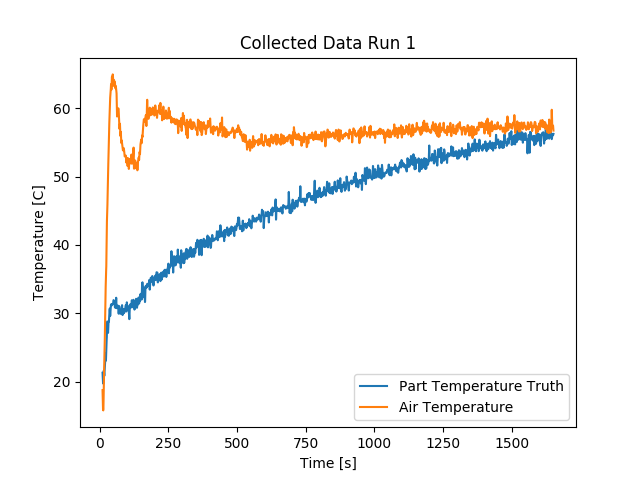
\includegraphics[width=\linewidth]{other/Raw_Data/1.png}
        \caption{Run 1}
    \end{subfigure}
    \begin{subfigure}{.33\linewidth}
        \centering
    	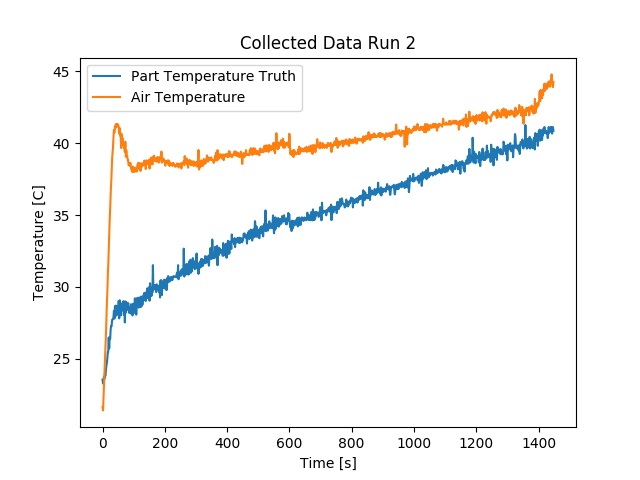
\includegraphics[width=\linewidth]{other/Raw_Data/2.png}
    	\caption{Run 2}
    \end{subfigure}
    \begin{subfigure}{.33\linewidth}
        \centering
    	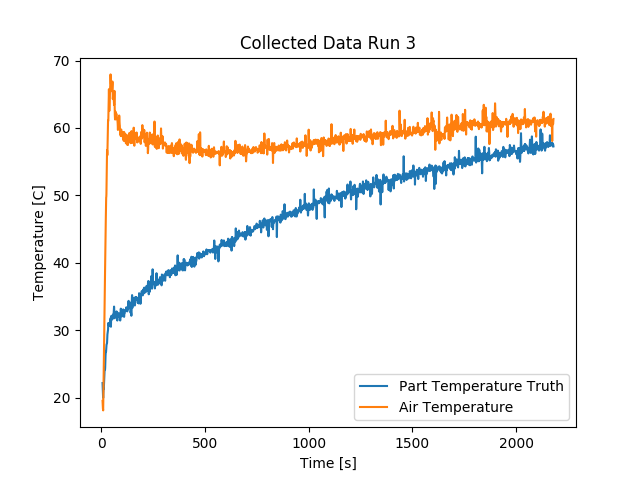
\includegraphics[width=\linewidth]{other/Raw_Data/3.png}
    	\caption{Run 3}
    \end{subfigure}\par\medskip
    \caption{Data Collected from Runs 1 to 3}
    \label{fig:real_data0-3}
\end{figure}

\subsection{MATLAB Data Generation}
Here the methods for creating the MATLAB transient heat simulations for this project are explained and their results are examined. The general methodology used for generating these simulations are discussed. The specific toolboxes, functions, and strategies implemented in MATLAB are then described in this section. \\\\
The purpose of generating transient heat simulations is so the resulting data can be used for testing and training our machine learning models. Through research and investigation we found that MATLAB could be implemented for generating data sets using its finite element analysis features for modelling heat transfer problems. Building these heat simulations also made it feasible to study different materials, geometries, and temperature distributions. 

\subsubsection{Governing Equations}
For our transient heat simulations it was important to understand the governing equation that models the heat transfer problem. Using the approximation of a rectangular block revolved around the central axis, an idealized thermal equation was needed to create the simulations. Equation \ref{equation_matlab} shows the PDE used to model the transient conduction for the heat transfer problem. With T being temperature, $\rho$ is material density, $C_{p}$ is the specific heat value, $k$ is the thermal conductivity, and $f$ is the heat generated inside the cylinder. This equation is temperature dependent and is used to govern the heat conduction through the cylinder. 
\begin{equation}
    \rho C_p \frac{dT}{dt}   - \nabla \cdot (k \nabla T) = f 
    \label{equation_matlab}
\end{equation}

\subsubsection{MATLAB Simulated Data Generation}
First, using the \lstinline{createpde} function a PDE model of the system is created and it also sets up a transient simulation on this PDE model. Next, the geometry of the cylinder and the surrounding shape of the air is programmed. The geometry of the cylinder was approximated by using a 2D rectangle and revolving it around its central axis would then create a cylinder. This geometry is enclosed with boundary conditions set to represent the surrounding air inside the heating chamber. In Figure \ref{fig:matlab_heatchamber} this model is plotted showing the cylinder and the surrounding air with their position along the X and Y axes. This model also has the thermal properties programmed for the air and aluminum cylinder so the thermal conductivity across the cylinder can then be simulated. Then the temperature conditions were set to heat from the boundaries or edges ‘E1, E2, E6, E7’ of Figure \ref{fig:matlab_heatchamber} which gave a realistic simulation of the infrared lamp heating the cylinder from all directions. The \lstinline{transientBCHeatedBlock} function was used to set the initial, rise, and final temperatures on these edges. This function allowed us to set the temperature conditions for the simulation to mimic the curing cycles in the physical heating chamber experiments as accurately as possible.
\begin{figure}[!htb]
    \begin{subfigure}{.5\linewidth}.
        \centering
        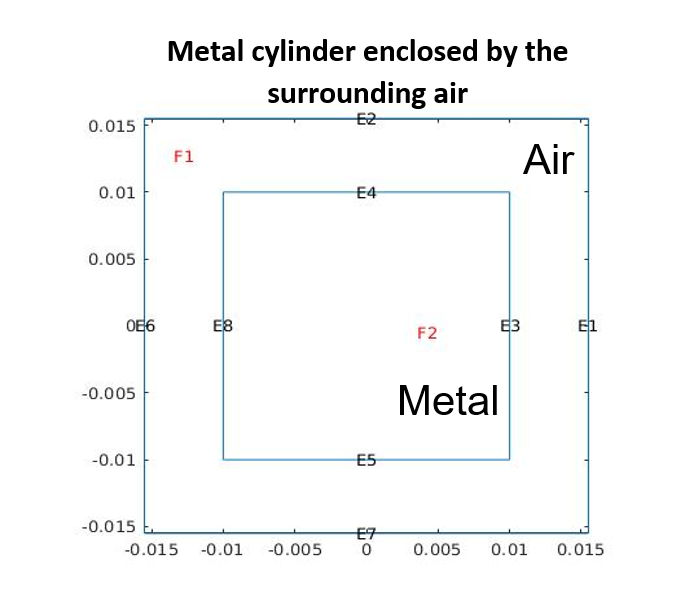
\includegraphics[width=0.65\linewidth]{other/metal_cylinder_mesh.png}
        \caption{Mesh of Metal Cylinder Approximation}
        \label{fig:matlab_heatchamber}
    \end{subfigure}
    \begin{subfigure}{.5\linewidth}.
        \centering
        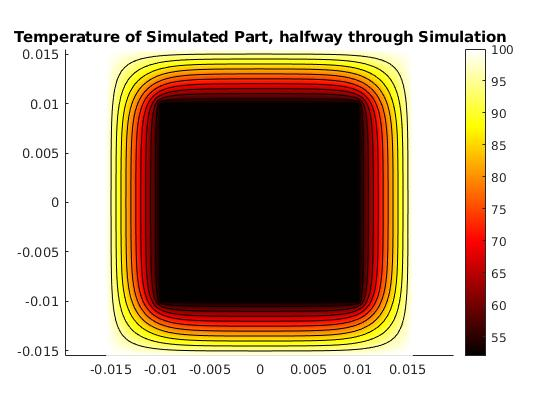
\includegraphics[width=0.7\linewidth]{other/transient_solution.png}
        \caption{Heat Distribution from Simulation}
        \label{fig:transient_solution}
    \end{subfigure}
    \caption{Heat Chamber Simulations using MATLAB}
\end{figure}

Having the model geometry, material properties, and boundary conditions symmetrical about the central axis also created a uniform heat distribution across the simulated cylinder. %It was known from experimental testing that the center of the cylinder heated up slower than the outer surface due to the aluminum’s thermal conductivity.
For the simulations a PDE with constant thermal conductivity and material properties not temperature dependent were assumed. %This was based on experimental observations of the conductive heat transfer through the material. The assumption is seen in the MATLAB script with the thermal conductivity value being set as a constant throughout the simulation. 
Combining the external air temperature conditions with this constant thermal conductivity assumption produced a representation of the cylinder’s internal temperature over time. 
The results from Figure \ref{fig:transient_solution} shows the simulation halfway through where there is a uniform heat distribution across the cylinder which is lagging behind the air temperature which is at 100$^\circ$C.

\subsubsection{Transient Heat Simulation Outputs}
The last part of these MATLAB simulations was to generate the transient response of the model and evaluate the outputs. This was easily done using more built-in functions in the PDE toolbox. In MATLAB, the simulations were programmed to capture the temperatures at the air boundary and the center of the cylinder. The simulation is also set to save the temperature data every 1 second over the entire heating cycle. Then when the code is run, multiple time series data sets are produced showing ideal curing cycles. An example of a simulated curing cycle generated with MATLAB is shown in Figure \ref{fig:comparison_sim_real}a with a maximum curing temperature of 85$^\circ$C. Then in Figure \ref{fig:comparison_sim_real}b the curing cycle of a real data set is shown with maximum temperature at 60$^\circ$C. The MATLAB data set shows the air temperature’s curve having a more gradual rise compared to the curve from the heat chamber data set. This due to the settings of the PID controller in the heat chamber programmed to ramp up faster than the simulation. However, the simulations still provide robust data for training machine learning algorithms which will be able to predict the heat chamber conditions when fed experimental data after being trained on these simulated data sets.\\\\
The MATLAB transient heat simulations satisfied their overall purpose of generating multiple data sets with varying parameters. It was possible to change parameters like shape, material, conductivity of air, and temperature conditions without doing time-consuming experimental runs in the laboratory. The MATLAB code also has the ability to perform the simulations with different parameters in parallel. The parallelization of the data generation code reduced the runtime for generating 20 data sets from 1.5 hours down to approximately 15 minutes. 

\begin{figure}[!htb]
    \begin{subfigure}{.5\linewidth}.
        \centering
    	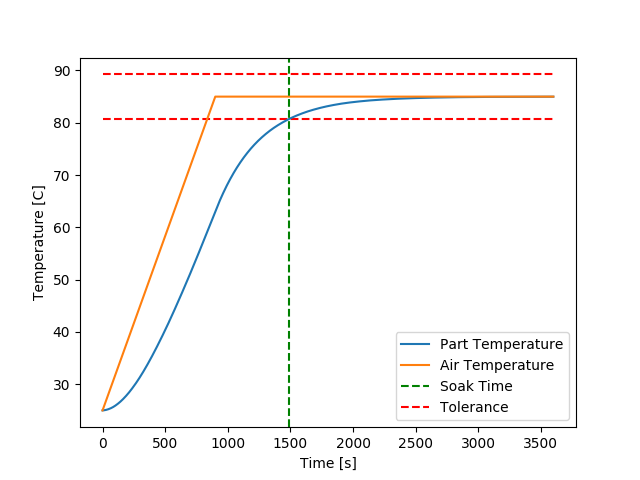
\includegraphics[width=0.9\linewidth]{other/sim_data.png}
        \caption{Simulated Data with a 5\% tolerance marked and soak time}
    \end{subfigure}
    \begin{subfigure}{.5\linewidth}.
        \centering
    	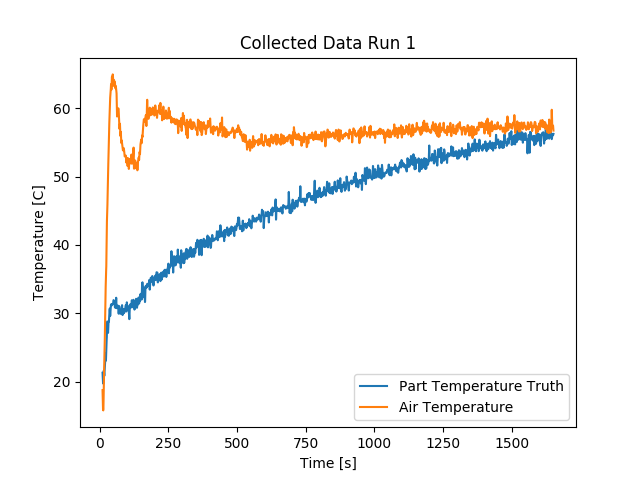
\includegraphics[width=0.9\linewidth]{other/Raw_Data/1.png}
        \caption{Curing Cycle using Real Dataset}
    \end{subfigure}
    \caption{Comparison of Simulations and Real Data}
	\label{fig:comparison_sim_real}
\end{figure}
\clearpage

\subsection{Data Filtering}
In this project, it was in our interest to understand the effects of noise from our temperature sensors on the machine learning process. We wanted to know if noise from the sensors was affecting the soak time estimate and if noise would affect the accuracy of the prediction by the machine learning methods, as the data to train on would be more inconsistent with noise present. To perform our analysis, we began by running our data through various filters: A Savitzky-Golay filter and a Kalman filter, both implemented in Python. A Savitzky-Golay filter was chosen because it is an effective filter for smoothing data through local regression and can be implemented with ease. The Savitzky-Golay filter is more sensitive to bursts of noise and therefore has the possibility of skewing the signal, however it seemed like an appropriate fit due to the uniformity of our data. A comparison of the filtered data using Savitzky-Golay filter and the unfiltered data can be seen in Figure \ref{fig:savitzky} below. It can be observed that despite some inaccuracy located after the initial rise in temperature, the filter was effective in smoothing the data. Following this, we ran our sample data through a Kalman filter. For our application, the Kalman filter was used to extract the signal from the noise, which provided us with a significantly more accurate representation of the signal with smaller noise margins. The Kalman filtered data and the unfiltered data are compared in Figure \ref{fig:kalman}. The filter was ultimately able to fulfill our intended application.\\\\
To test our concerns, we trained our machine learning methods and performed predictions using unfiltered data, the Savitzky-Golay filtered data, and the Kalman filtered data. We then performed a comparative analysis on the soak time estimates of each prediction and the accuracy of each prediction relative to the true temperature of the cylinder. The figures below demonstrate the predictions from the aforementioned data through the LSTM method and the Random Forests method, respectively, for one sample run from our data set. From our analysis, we observed minor improvements through filtering the data with the Kalman filter, with similar albeit not as improved results using the Savitzky-Golay filter regarding the accuracy of the predictions. We did not observe any difference in the estimated soak time from filtering the data. We were ultimately able to conclude that the effects of noise are mostly negligible for the project application, as the noise did not have any significant impact on the machine learning process or the soak time. Further data analysis in this report is performed with the Kalman filtered data, as it provides a more visually informative and accurate view of the relationships between the curves in plotting.

\begin{figure}[h]
    \begin{subfigure}{.5\linewidth}.
        \centering
    	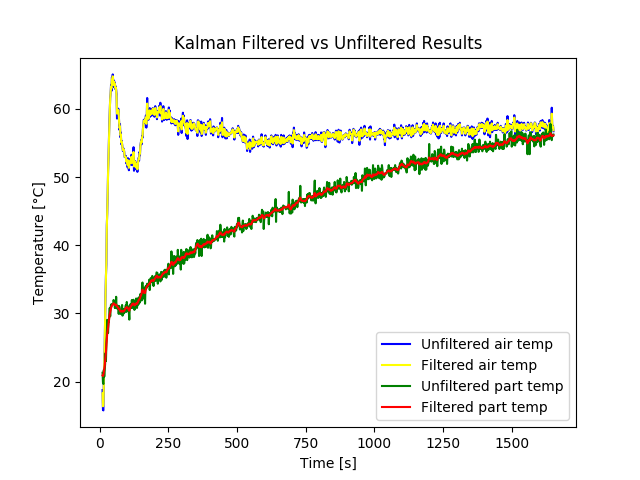
\includegraphics[width=1\linewidth]{filter/kalman.png}
        \caption{Kalman Filtered Data}
        \label{fig:kalman}
    \end{subfigure}
    \begin{subfigure}{.5\linewidth}.
        \centering
    	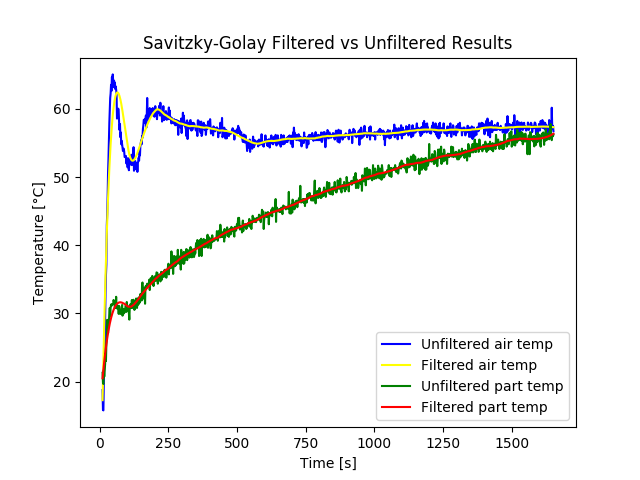
\includegraphics[width=1\linewidth]{filter/savitzky.png}
        \caption{Savitzky-Golay Filtered Data}
    	\label{fig:savitzky}
    \end{subfigure}
    \caption{Data Filtering Techniques}
\end{figure}
\begin{figure}[ht]
    \vspace{-0.9cm}
    \begin{subfigure}{.34\linewidth}.
        \centering
    	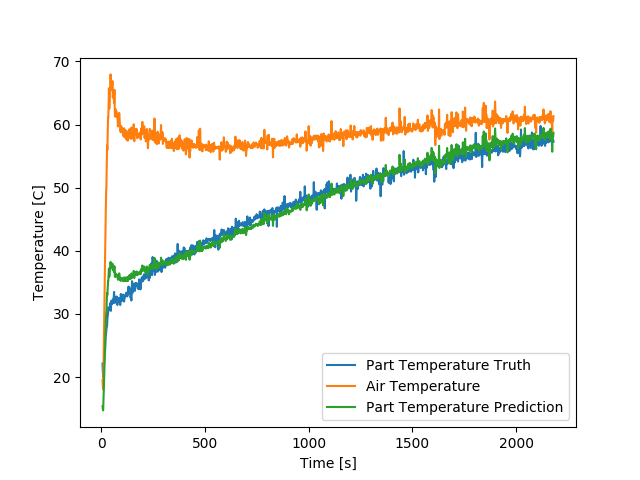
\includegraphics[width=1.1\linewidth]{filter/unfiltered_LSTM.png}
        \caption{Unfiltered Data with LSTM}
    \end{subfigure}
    \begin{subfigure}{.34\linewidth}
    	\centering
    	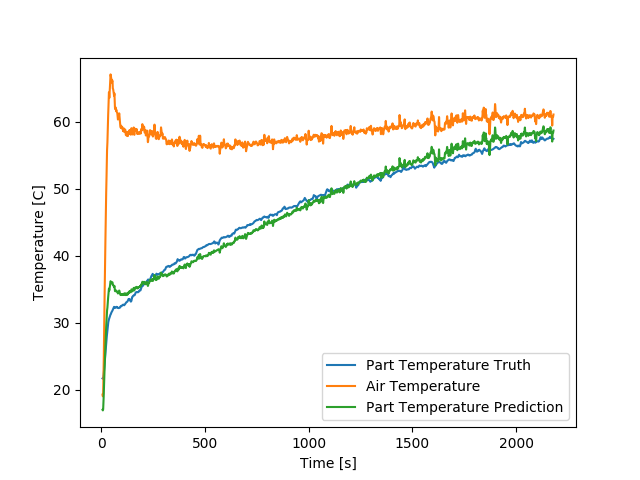
\includegraphics[width=1.1\linewidth]{filter/kalman_LSTM.png}
        \caption{Kalman Data with LSTM}
    \end{subfigure}
    \begin{subfigure}{.34\linewidth}
    	\centering
    	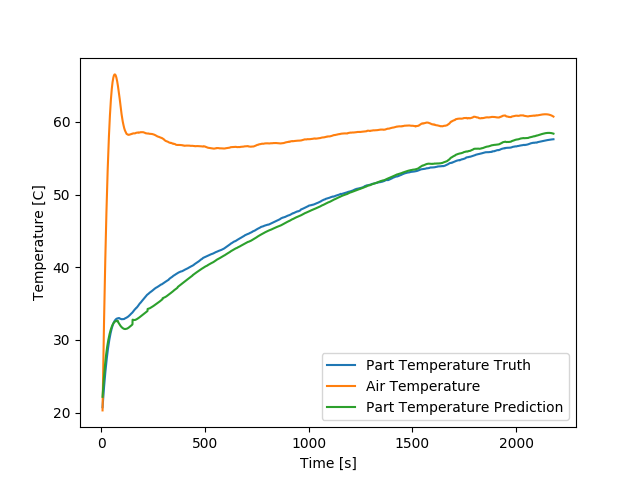
\includegraphics[width=1.1\linewidth]{filter/savitzky_prediction_LSTM.png}
    	\caption{Savitzky Data with LSTM}
    \end{subfigure}
    \caption{Predictions using Filtered Data with LSTM}
\end{figure}

\begin{figure}[ht]
    \begin{subfigure}{.34\linewidth}.
        \centering
    	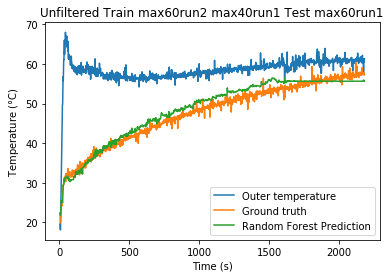
\includegraphics[width=\linewidth]{filter/unfiltered_RF.png}
        \caption{Unfiltered Data with Random Forest}
    \end{subfigure}
    \begin{subfigure}{.34\linewidth}
    	\centering
    	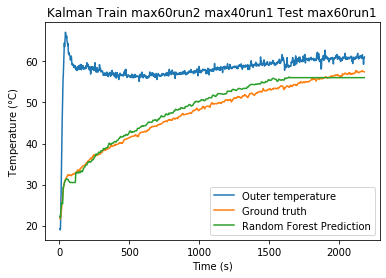
\includegraphics[width=\linewidth]{filter/kalman_RF.png}
        \caption{Kalman Data with Random Forest}
    \end{subfigure}
    \begin{subfigure}{.34\linewidth}
    	\centering
    	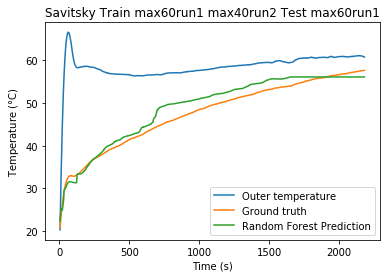
\includegraphics[width=\linewidth]{filter/savitzky_RF.png}
    	\caption{Savitzky Data with Random Forest}
    \end{subfigure}
    \caption{Predictions using Filtered Data with Random Forest}
\end{figure}\clearpage
\subsection{Data Scaling}
To input the data into a neural network, it improves performance to manipulate the data and scale it between values of 0 and 1. Large inputs which are disproportionate to each other can slow down the convergence of the training algorithm and can in some cases prevent the neural network from classifying the problem \cite{hands_on_scaling}. A \lstinline{min_max} function is used to scale the input data between ranges min and max, which are commonly set to values 0 and 1 respectively. 
\begin{equation} \label{scaled_eq1}
    X_{std} = \frac{(X - X_{min})}{(X_{max} - X_{min})}
\end{equation}
\begin{equation} \label{scaled_eq2} 
    X_{scaled} = X_{std} (max - min) + min
\end{equation}

Time, if desired as an input feature to the neural network, can be scaled from 0 to 1 signifying the duration of the run from  start to finish. As all runs follow a predictable start and finish, where at the start part temperature is equal to air temperature and at the end of the run the same is true. The time data can then be a feature which shows where in the run the network is, and if needed expanded beyond 1 to predict future data which has never been seen by the neural network. Temperature data can be scaled so the minimum temperature across all runs training runs is the minimum value used in equation \ref{scaled_eq2}, and the max temperature value across all training runs is the value used in  \ref{scaled_eq2}. The scaling is shown below in Figure \ref{fig:scale1}. It can be seen that the two runs which were set to 60$^\circ$C are similar in nature and the run which is set to 40$^\circ$C is obviously lower. Time is scaled from 0 to 1. All runs are interpolated to be the same size which is used for the LSTM network.\\
\begin{figure}[h]
    \centering
    \vspace{-25pt}
    \centerline{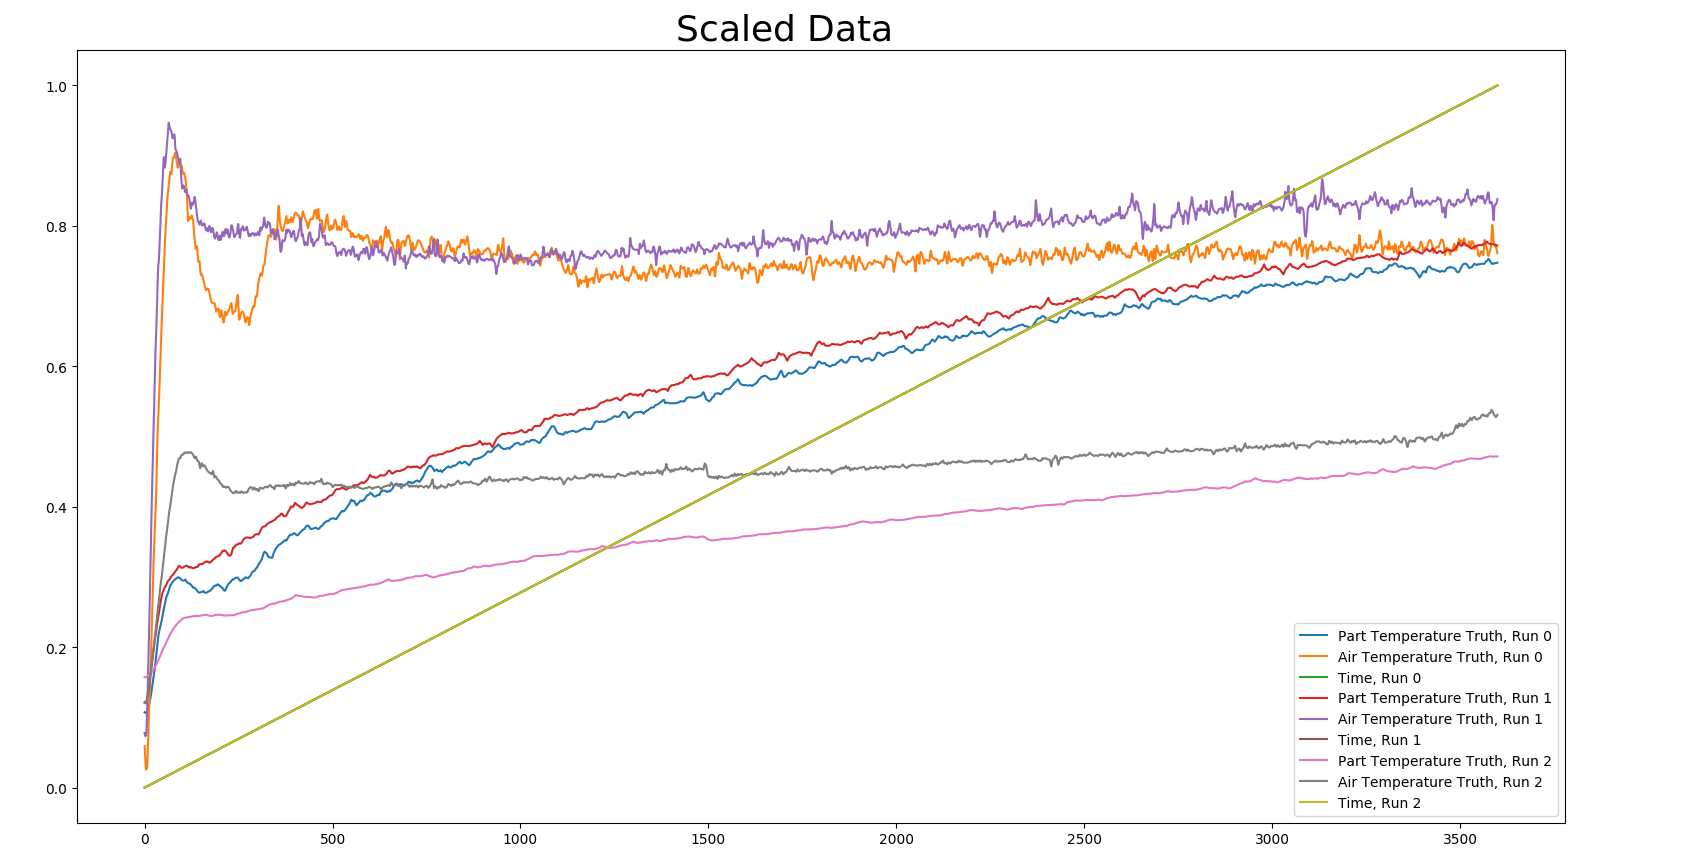
\includegraphics[width=0.9\linewidth]{scaling/image1.png}}
    \caption{Scaling Input Features Part and Air Temp, and Time using Predefined Constants for Temperatures}
    \label{fig:scale1}
\end{figure}
\newpage
%Alternatively, temperature can be scaled on a per run basis, meaning that the max and min are set per run and not as a max/min for all runs. The result is a series of similar curves which all follow the same slope and value profile which is shown below in Figure \ref{fig:scale2}. The main disadvantage is that this method loses the scale of the temperature and instead just shows how it changes during a run. In the end, this method produces greater error and was not used as the scaling lost essential data, as the neural network does not know that run 2 was the lowest temperature run which resulted in the part temperature rising the slowest. This method could be useful if temperature was not a feature that changed between runs or if time series temperature data itself held some kind of slope which implied a higher or lower temperature. This scaling might be used if one wanted to reduce training time and get a result which is more general.
%\begin{figure}[htb]
%    \centering
%    \centerline{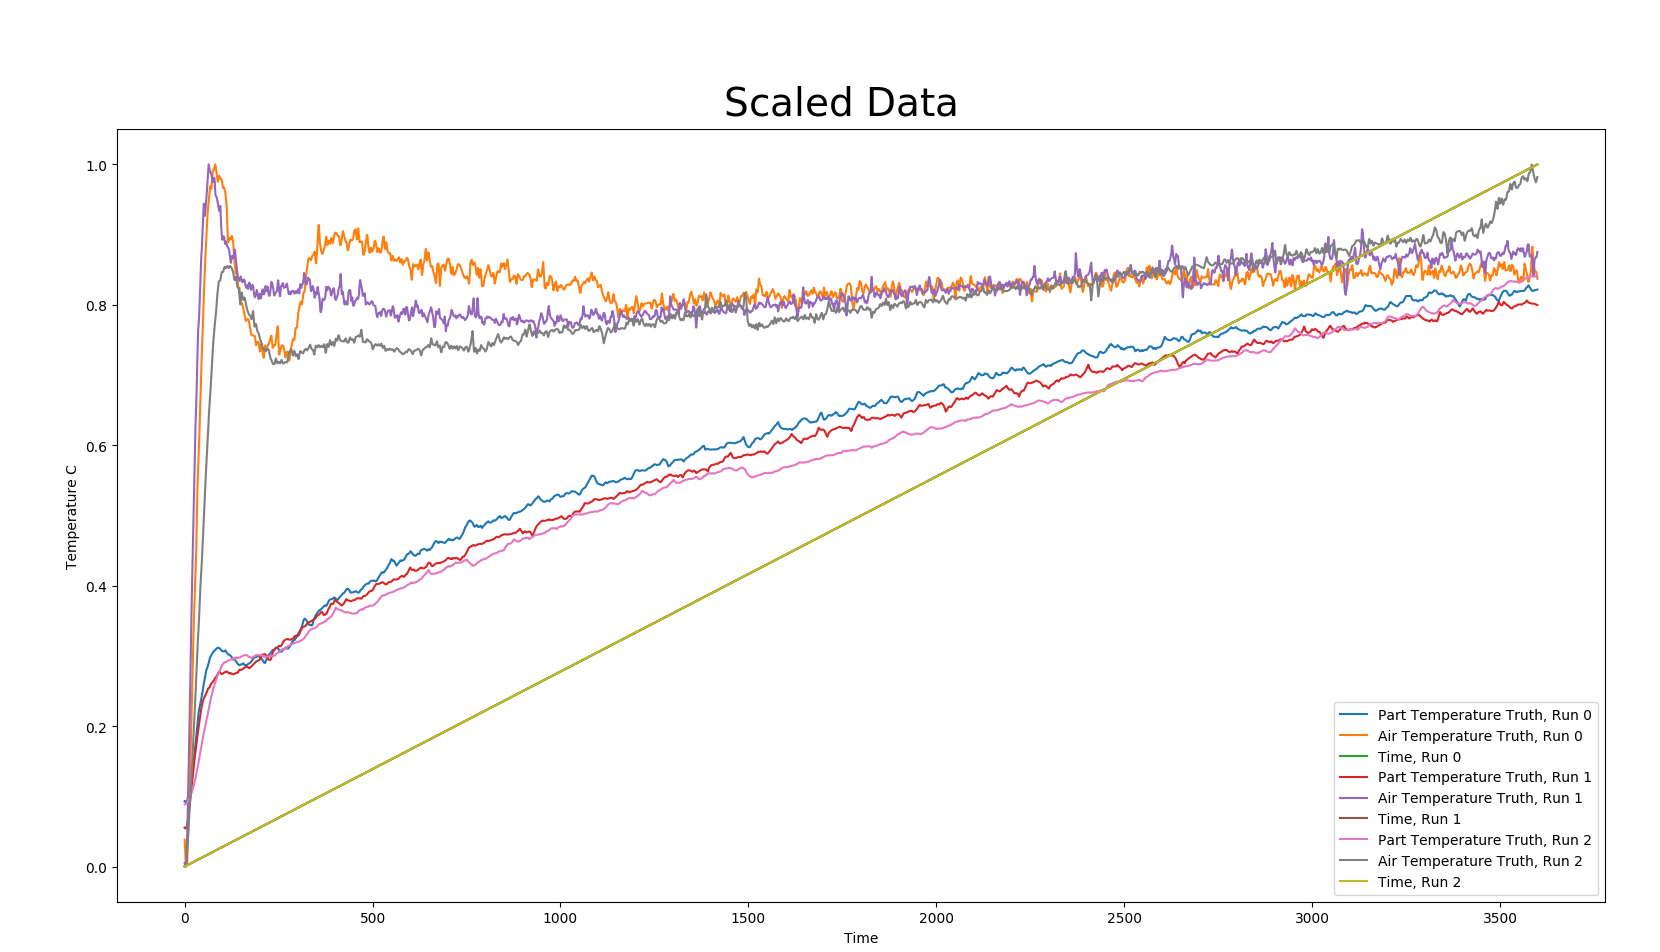
\includegraphics[width=0%.9\linewidth]{scaling/image12.png}}
%    \caption{Scaling Input Features %using Maximums and Minimums}
%    \label{fig:scale2}
%\end{figure}
\subsection{Recurrent Neural Networks}
RNNs are particularly powerful for time series prediction and classification, employing the linear and unidirectional nature of time to achieve better predictions. RNN, like other neural networks, are at the most basic level a collection of obfuscated neurons which when given an input perform arithmetic operations mainly weighting and biasing to give an output. RNN are different, in that they introduce a feed backward implementation which takes an output time step and reintroduces this as an input. The simplest is a single neuron which receives inputs and sends the output back to itself as a new input. Extending this concept, multiple neurons can be chained together with each output feeding to a neighboring neuron based on time. This version forms neuron connections aligned temporally based on the input time-steps. This is shown in Figure \ref{fig:lstm_dia} with the simplest case on the left containing one neuron and a chain of neurons on the right. One of these yellow boxes can be implemented as a layer of neurons so that a layer of neurons feedback to a neighboring layer of neurons. Due to the action of feedback, RNNs can be thought of as having memory where past inputs are recalled as they are propagated through the chain of neurons. Many types of RNN neurons exist including standard RNN, LSTM, and GRU.

\begin{figure}[ht]
    \centering
    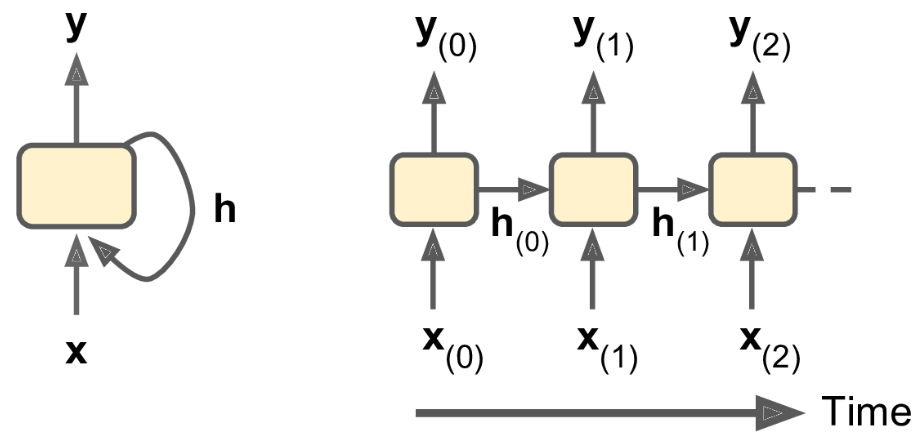
\includegraphics[width=.5\linewidth]{lstm/lstm_diagram.png}
    \caption{Block Diagram of a RNN}
    \label{fig:lstm_dia}
\end{figure}

\begin{comment}
Each neuron contains two sets of weights one which is used for the input and the other which is used on the feedback. Figure \cite{rnn_node} shows these weights as input weight (IW), and the delay weight (LW). The delay weight takes a delayed input delayed by block D. Block b is a bias weight which can be thought of as an offset which is applied to each neuron. The addition of these weights are added and input through an activation function in green. An output layer is typically (always) added to the output of the RNN. 
\begin{figure}[h]
    \centering
    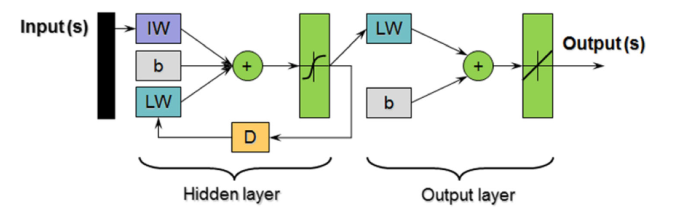
\includegraphics[width=.3\linewidth]{lstm/RNNnode.png}
    \caption{Block Diagram of a RNN}
    \label{fig:rnn_node}
\end{figure}
\end{comment} 

\subsection{Long Short Term Memory Networks}
LSTM networks are a particular subset of RNNs. The motivation and usage of an LSTM network are increased performance in long term dependencies in data at the cost of some additional computation power. An LSTM block takes an input $x_t$ and two states, the long term $c_{t-1}$ and short term $h_{t-1}$, which are used to determine the output state $h_t$ which is sent to the output layer. Three gates regulate information through the LSTM dropping or allowing memories based on pointwise operation controlled by weights $\sigma$. Essentially, the LSTM attempts to recognize important input. The Forget weight controlled by $f(t)$ regulates long term memories which should be erased. Input gate controlled by $i(t)$ adds memories to the long term memory. Output gate controlled by $o(t)$ allows long term states to be read by the output layer and passed on.  The governing equations for the LSTM block are shown below taken from \cite{hands_on_lstm}. $W_{xi}, W_{xf}, W_{xo}, W_{xg}$ are all neuron weights for the cell.  $W_{hi}, W_{hf}, W_{ho}, W_{hg}$ terms are weights from the previous short term state. Terms $b$ are bias terms or offsets. $Tanh$ functions can be changed and are the activation functions of the LSTM cell. The long term memory output $c_t$ of the cell is a function of the Forget gate and new inputs through the input gate. The short term memory and output y(t) is determined by the activation of the previous output modified by the activation of the long term memory. These gates can be seen in Figure \ref{fig:lstm_neuron}. Essentially, the LSTM network implements gates to increase the stability of learning both short term and long term memories in time series data by allowing and dropping certain memories from the cell. 

\noindent\begin{minipage}{.55\textwidth}
   \centering
   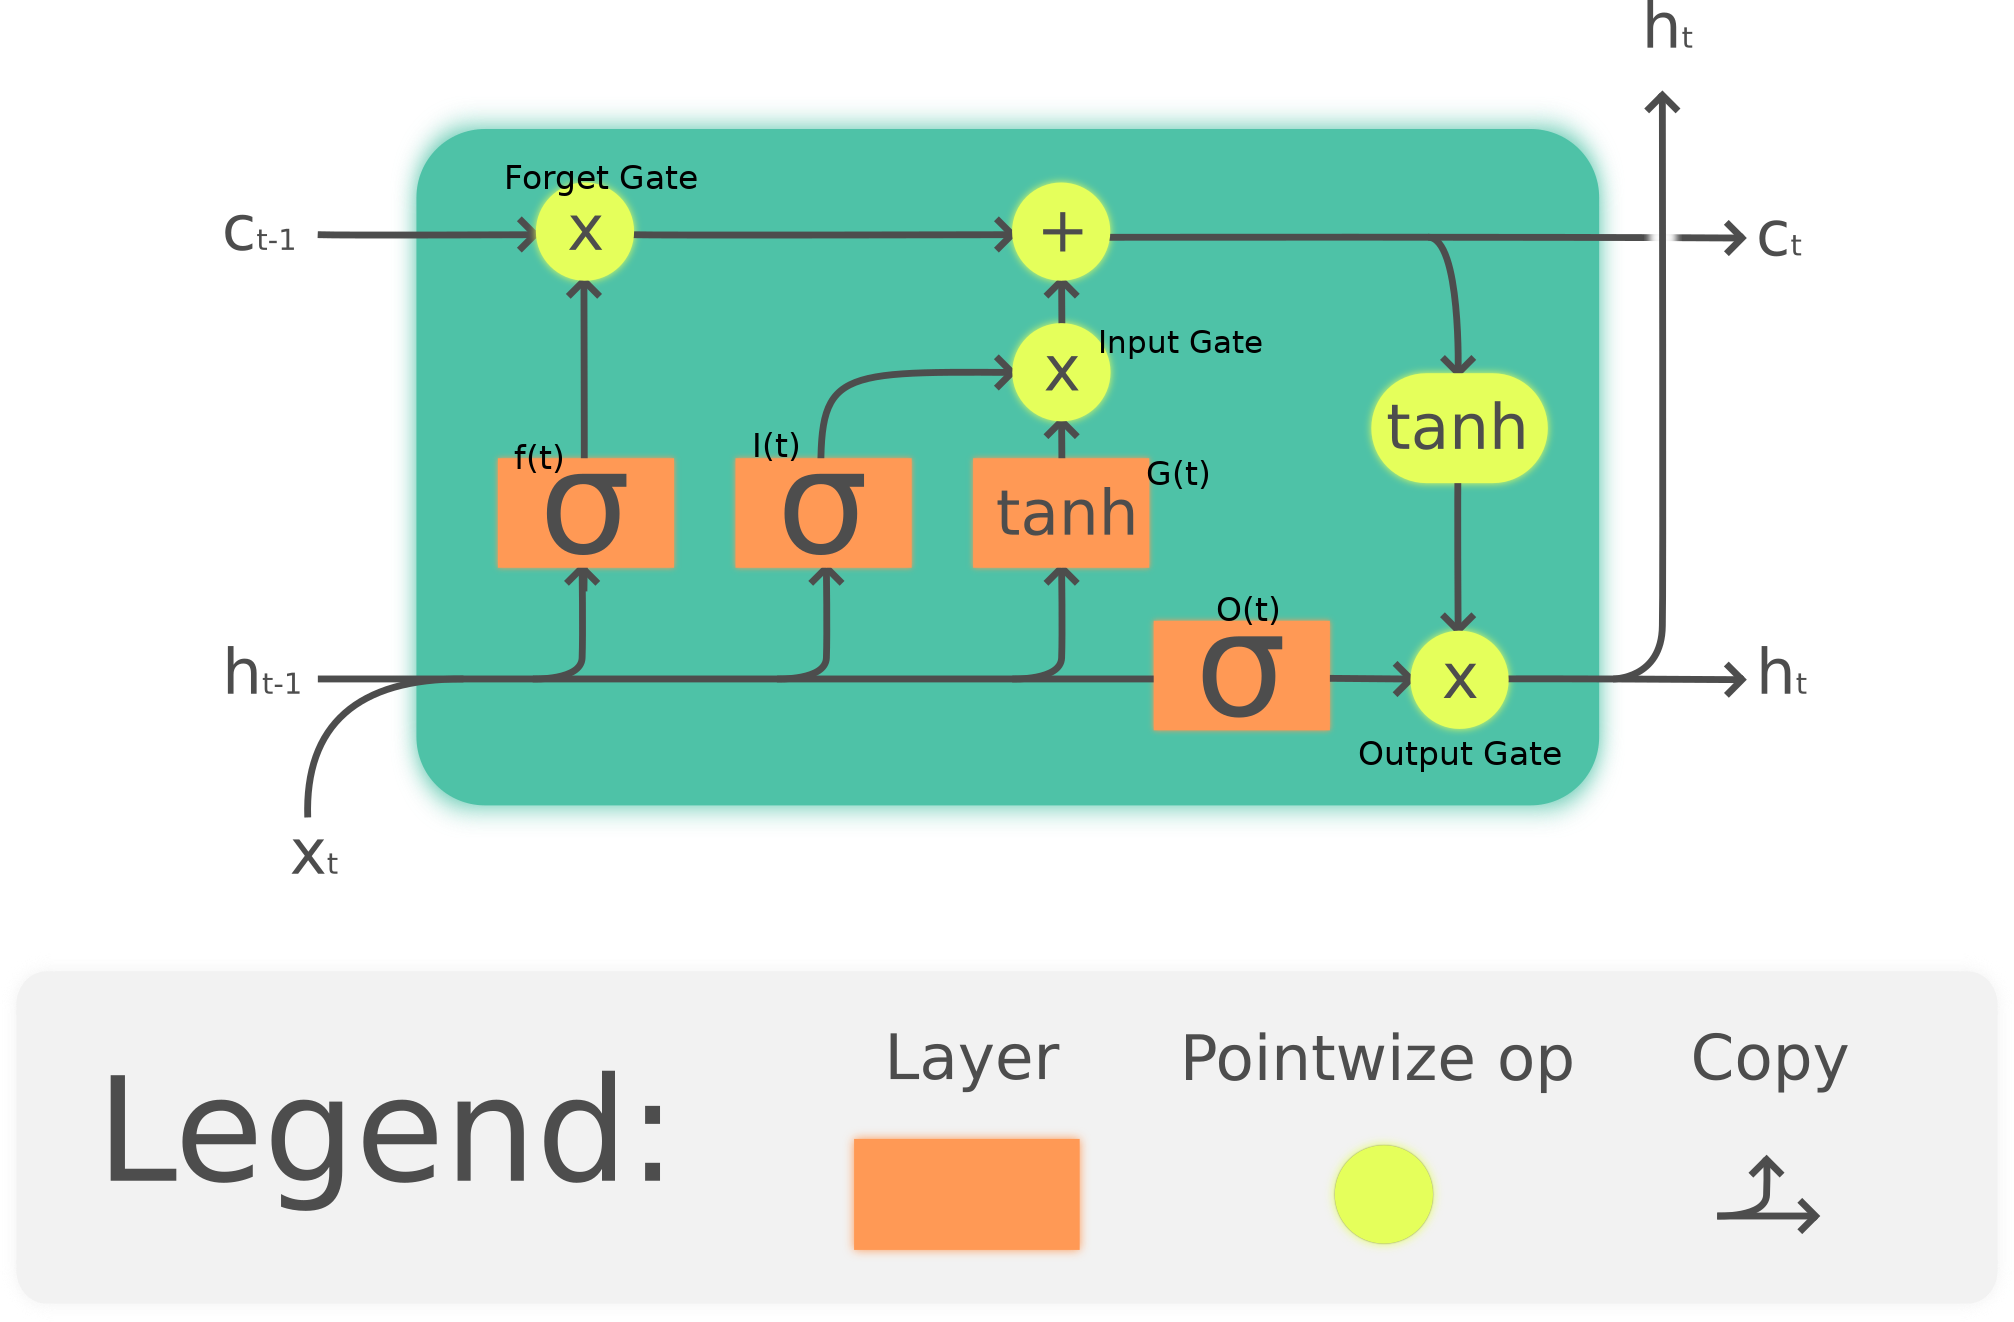
\includegraphics[width=\linewidth]{lstm/neuron_lstm.png}
   \captionof{figure}{Diagram of LSTM Neuron}
   \label{fig:lstm_neuron}
\end{minipage}
\begin{minipage}{.43\textwidth}
\begin{align}
        i(t) = \sigma(W_{xi}^Tx(t) + W_{hi}^Th(t-1) + b_i \\
        f(t) = \sigma(W_{xf}^Tx(t) + W_{hf}^Th(t-1) + b_f\\
        o(t) = \sigma(W_{xo}^Tx(t) + W_{ho}^Th(t-1) + b_o\\
        g(t) = tanh(W_{xg}^Tx(t) + W_{hg}^Th(t-1) + b_g\\
        c(t) = f(t) \bigotimes c(t-1) + i(t) \bigotimes g(t)\\
        y(t) = h(t) = o(t) \bigotimes tanh(c(t))
\end{align}
\end{minipage}

\subsection{LSTM Parameters}
Multiple different implementations were attempted to try and attain the lowest possible error. Two implementations were created, one using a simple method with a single feedback loop and another implementing data windowing. In addition to trying these two implementations, the parameters for each of these implementations were adjusted to attain the lowest possible loss on predicted data. 
\subsubsection{Simple LSTM}
 This method of LSTM network is the easiest implementation of an LSTM model which acts on time series data. The model acts on a single time step at a time, a diagram of the model is shown below in Figure \ref{fig:lstm_io}. The time of the run and the air data are fed into the neural network one time sample at a time. The output temperature data is fed back into the LSTM. The process repeats until all samples are consumed. The LSTM network is a collection of N neurons which are formed together to create a layer of LSTM cells which all receive the data and output the data. 
\begin{figure}[h]
    \centering
    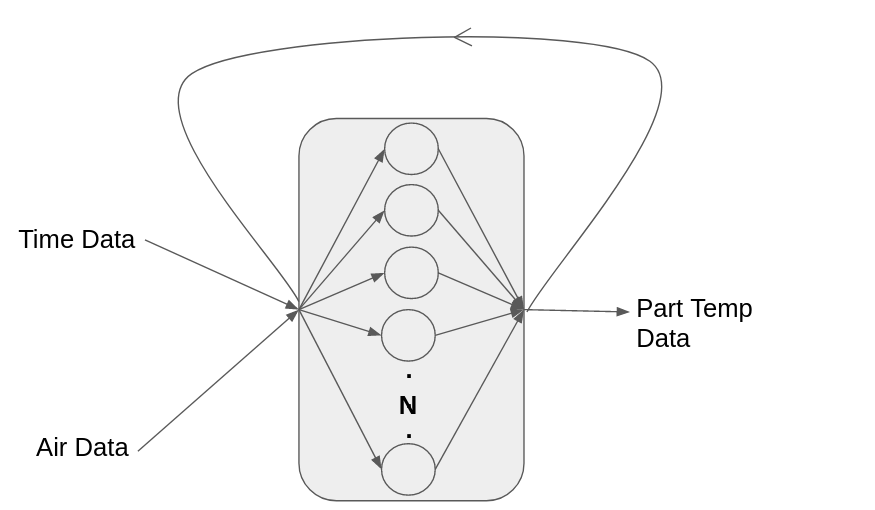
\includegraphics[width=.4\linewidth]{lstm/lstm_diagram_io.png}
    \caption{Input Output and feedback of LSTM layer}
    \label{fig:lstm_io}
\end{figure}
The time data and air temperature data is scaled to better accommodate the activation functions within the LSTM blocks which perform between the range of 0 and 1. The data varies in length but is set to 3600 in our LSTM networks to evaluate 60 minute runs with a single sample per second. In the case of the real data which is shorter than 3600 samples data is interpolated to increase its length. 
\subsubsection{Parameters} \label{lstmparameters}
The key parameters of the network include number of neurons, input dimension, dropout layer, and output layer. The LSTM layer consists of 25 neurons which take a three dimensional input array. Twenty-five neurons performed well on the data. A span between 10 to 50 resulted in fairly equal performance. The neurons are contained in a single hidden layer. Increasing the number of neurons has the possibility of over-fitting the data especially due to the low number of real runs that are available to train on. A higher number of neurons will also increase the training time. The network was set to ‘Stateful’ which means the network state is conserved through training batches. Through experimentation of different activation functions in the LSTM neuron, it was found that Softsign activation performs adequately. A Rectified Linear Unit (ReLU) activation also provided extremely similar performance. A dropout layer is added to the network to reduce over-fitting. The dropout layer thins the connections between neurons by randomly setting an input to a random neuron to zero depending on a certain rate \cite{dropout}. The rate is set to .0001 which is very low, as we are not overly concerned about over-fitting in our data set as the data set is so small it is almost unavoidable. An output layer is added to the LSTM network and adds a bias to the output of the LSTM layer and performs an activation function on it. A linear activation function was chosen for the output layer as it was found to be adequate, and changing to other activation functions produced worse predictions.
\subsubsection{Training}
The training optimizer used was Adam, it performed the best out of the ones tested including Adaptive gradient algorithm (AdaGrap) and Root Mean Square Propagation (RSMProp). Adam is the typical default optimizer used in machine learning algorithms \cite{learn_keras}. A slightly reduced learning rate of 0.0005 was used, which provided lower loss over the typical rate of .001. This is likely due to the network 'learning' the data more effectively, as opposed to over-fitting the data. The downside of reducing the learning rate is the network will take more iterations and more time to train. Each trial was trained on the LSTM network for a single epoch, then a new trial was selected from the training set and this was repeated until the loss was reduced adequately. The model is fit in batches meaning only portions of the data is given to the network at a time. Smaller batches can increase the stochasticity of the gradient descent during training  which can allow the algorithm to jump out of local minima and find the proper minimum for the network \cite{learn_keras}. A batch size of around 180 samples was found to be adequate. To calculate the loss, the mean-squared-error (MSE) loss function was used. This loss function is the standard and provides a harsh loss compared to other functions meaning small deviations will produce a higher relative loss. The loss function is shown in Equation \ref{lstm_loss}. It was found that moving to other loss functions always produced worse prediction capability. Usual training took up to 1000 epochs before the loss stopped being reduced on the validation set.
\begin{equation}\label{lstm_loss}
    \text{MSE} = \frac{1}{n}\sum^n_{i=1}(Y_i - \hat{Y}_i)^2
\end{equation}
 The loss during training of the network is shown in the figure below. It can be seen that the loss drops quickly at first and then slowly later, and the test loss is higher than the training loss. The network takes under 15 minutes to train on an Intel$^{\textregistered}$ Core$^{TM}$ I5-4760k 4core 3.4GHz Processor with time depending on the amount of training data used. 
\begin{figure}[h]
    \begin{subfigure}{.5\linewidth}.
        \centering
    	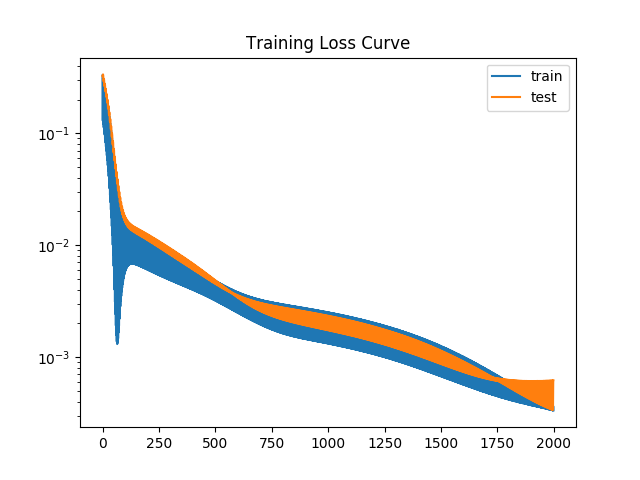
\includegraphics[width=\linewidth]{lstm/loss_f.png}
        \caption{Loss Curve 2000 epochs}
    \end{subfigure}
    \begin{subfigure}{.5\linewidth}.
        \centering
    	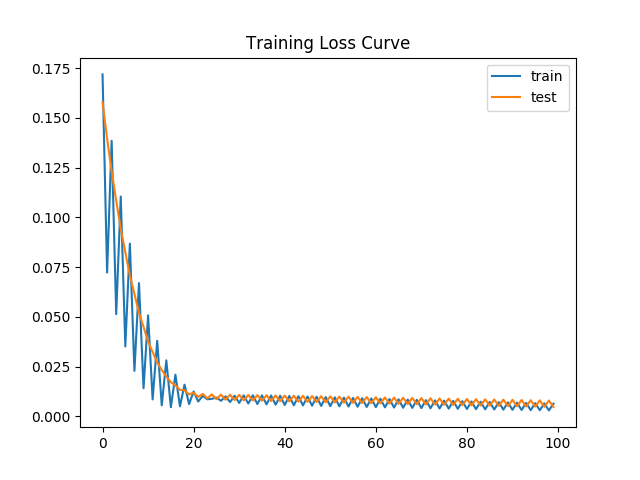
\includegraphics[width=\linewidth]{lstm/loss_2.png}
        \caption{Loss curve 100 epochs}
    \end{subfigure}\par\medskip
    \caption{Loss Graphs using MSE}
	\label{fig:loss}
\end{figure}

\subsubsection{Simple LSTM Simulated Data Performance}
The simulated data is a good case where there is a large pool of data and an interpolation is made on unknown data. The data is presented below in Figure \ref{fig:simulated_data_lstm}a. The machine learning algorithm shows a choppy output and the batch size can be seen where the machine learning algorithm was trained in batches. The error is low for all runs except for the first run shown in Figure \ref{fig:simulated_data_lstm}b but it can be seen that even this run is sufficient enough to make a prediction on soak time. It was also found that the performance could be vastly improved on simulated runs by scaling the temperature of trials using an individual max and min found from solely that trial. This would result in every temperature curve starting at 0 and ending at 1, and the rise of the part temperature would be extracted solely from the rise of the air temperature. Doing this kind of scaling would result in worse performance on real data as the air temperature does not exhibit a similar rise, so it was not used. 
\begin{figure}[ht]
    \begin{subfigure}{.5\linewidth}.
        \centering
    	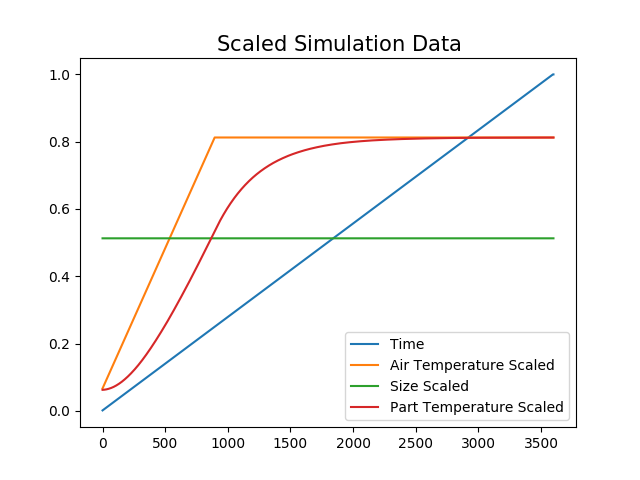
\includegraphics[width=\linewidth]{lstm/sime_data_scaling.png}
        \caption{Scaled Simulated data Input Features and truth}
    \end{subfigure}
    \begin{subfigure}{.5\linewidth}
    	\centering
    	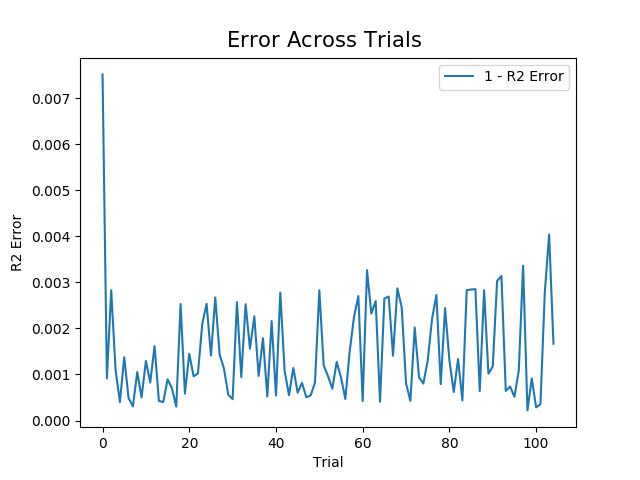
\includegraphics[width=\linewidth]{lstm/error.png}
    	\caption{Loss Across Runs R2 Error}	
    \end{subfigure}\par\medskip
    \begin{subfigure}{.5\linewidth}.
        \centering
    	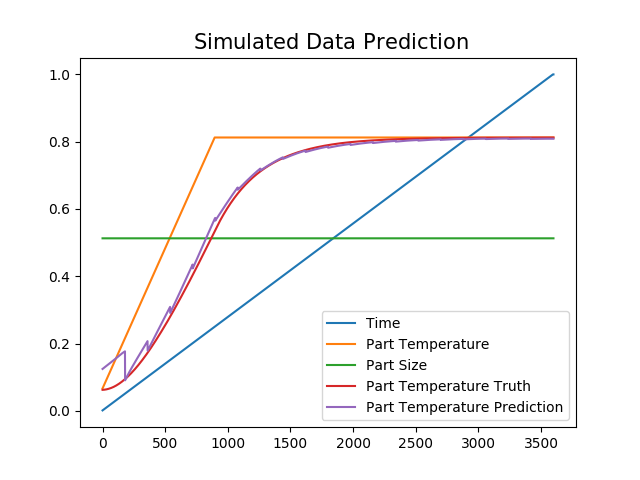
\includegraphics[width=\linewidth]{lstm/worst_sim_data.png}
        \caption{Highest Loss Run}
    \end{subfigure}
    \begin{subfigure}{.5\linewidth}
    	\centering
    	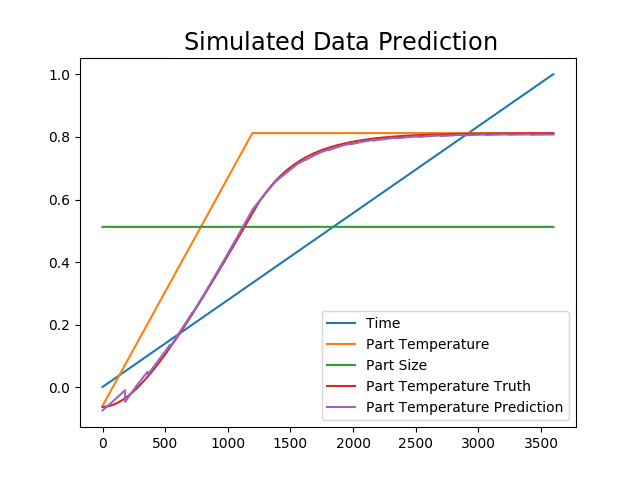
\includegraphics[width=\linewidth]{lstm/good_sim_data.png}
    	\caption{Average Loss Prediction}
    \end{subfigure}
    \caption{Simulated Data Information}
    \label{fig:simulated_data_lstm}
\end{figure}
\newpage
\subsubsection{Simple LSTM Real Data Performance} \label{simple_perf}
Real data was input two runs at a time and a prediction was then made on the third run. The summary of predictions is shown below in Figure \ref{fig:real_data_perf_lstm}. The predictions are better when stateful is set to false, most likely because the air data has a lower impact on the part temperature in the real data. The prediction of the 40$^\circ$C run by training on two 60$^\circ$C runs was poor due to the fact that no similar data was used to train and there was a limited amount of data to train on. 
\begin{figure}[ht]
    \begin{subfigure}{.34\linewidth}.
        \centering
    	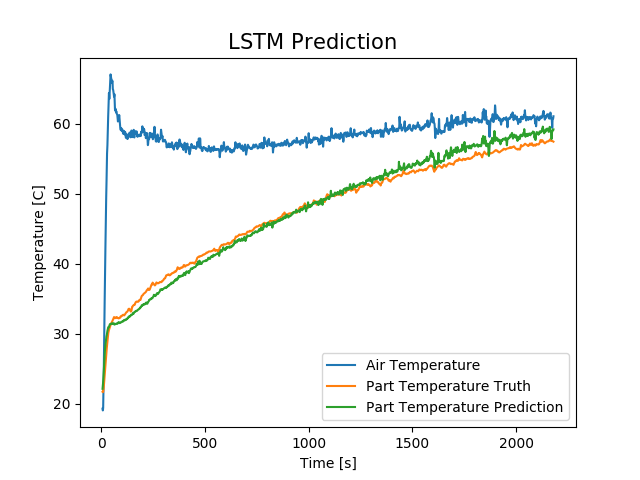
\includegraphics[width=\linewidth]{lstm/perf.png}
    \end{subfigure}
    \begin{subfigure}{.34\linewidth}
    	\centering
    	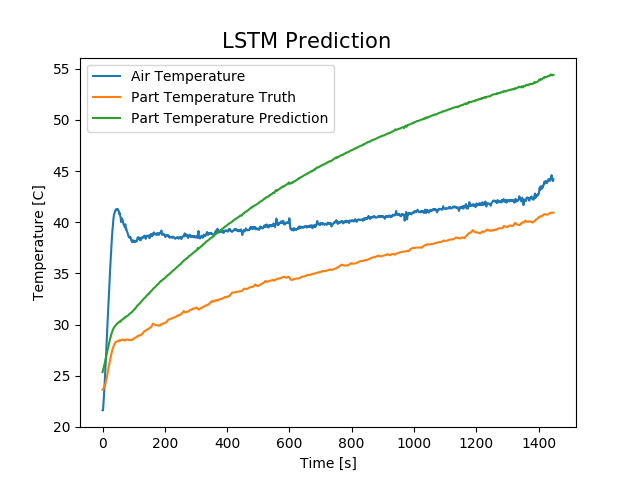
\includegraphics[width=\linewidth]{lstm/perf2.png}
    \end{subfigure}
    \begin{subfigure}{.34\linewidth}.
        \centering
    	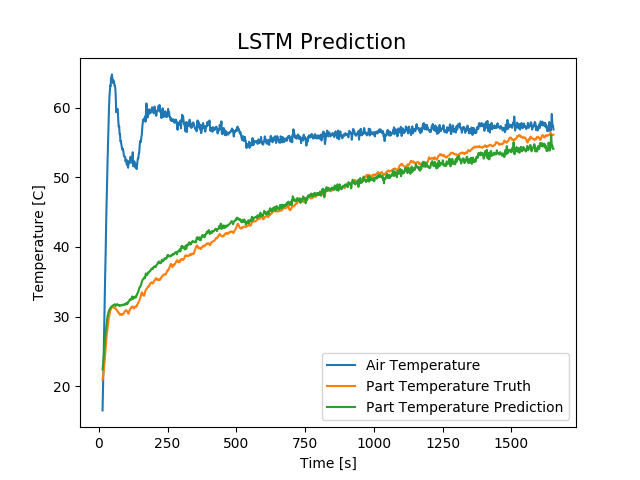
\includegraphics[width=\linewidth]{lstm/perf3.png}
    \end{subfigure}
    \caption{Real Data Predictions}
    \label{fig:real_data_perf_lstm}
\end{figure}
\newpage
\subsubsection{LSTM Windowed}
In an attempt to improve upon the simple LSTM model outlined above, another LSTM model was created using multiple time steps to make a decision. Unrolled, this model would be like the network below on the right. The network shares similar parameters to the other simple LSTM network. This network takes longer to train but can result in better predictions. The parameters used for the windowed method are the same as above and can be found in section \ref{lstmparameters}. 
\subsubsection{Windowed Data}
\begin{wrapfigure}{r}{0.5\textwidth}
  \vspace{-50pt}
  \begin{center}
    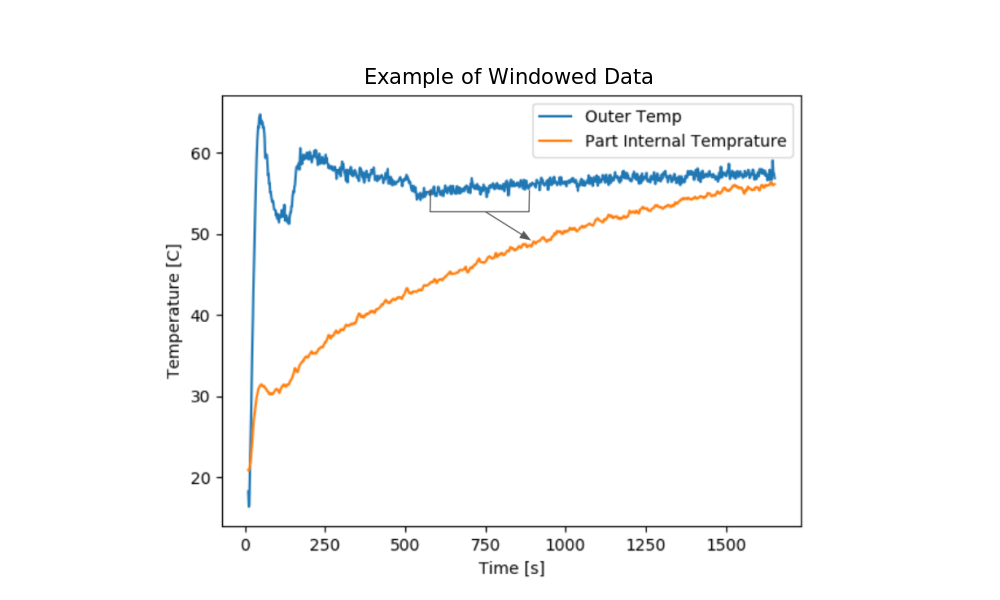
\includegraphics[width=0.6\textwidth]{lstm/window.png}
  \end{center}
  \vspace{-20pt}
  \caption{The window of data underlined which would be used to predict a single sample of part data which the arrow is pointing too}
  \label{fig:windowed}
  \vspace{-50pt}
\end{wrapfigure}
Windowed data is a way of organizing input features of the neural network to input samples and feed time data forward. The window implements a collection of data of past t-1 to t-N samples which are used to make a prediction on sample t. N can be any value, for our implementation a 50 sample window was chosen. An example of a window of data pointing at part temperature is shown in Figure \ref{fig:windowed} to the right, demonstrating what a window of data attempts to do. 

%\begin{figure}[h]
%    \centering
%    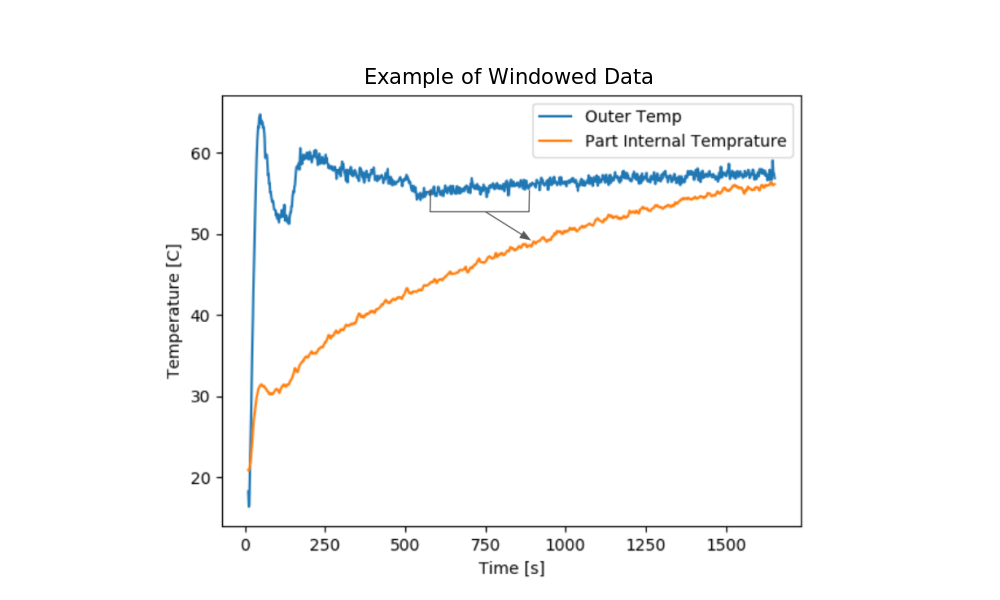
\includegraphics[width=.8\linewidth]{lstm/window.png}
%    \caption{Windowed Data Example}
%    \label{fig:windowed}
%\end{figure}
\newpage
\subsubsection{Windowed Method Prediction on Real Data}
The windowed method predicts slightly better than the simple method and is able to more closely fit data that it is trained on. It may also over-fit the data more. A dropout layer can help prevent over-fitting of the data although with this small of a data set to train on it makes minimal difference. From looking at the runs, it seems that the data is being learned more than overfit. This is exemplified by the dependency that part temperature has on the external air temperature shown by the hump from 500s-1000s in Figure \ref{fig:real_data_window_lstm1}. The end of the run matches closely with a percent error below 2\%, which is important for determining the soak time. Using Equation \ref{r2} the $R^2$ score was found for the first run to be 0.9824 and 0.9834 for the second run. Below in Figure \ref{fig:real_data_window_lstm1} \& \ref{fig:real_data_window_lstm2} the predictions are shown. The 40$^\circ$C run was not shown as it has a similar poor performance as the simple LSTM method shown above in Figure \ref{fig:real_data_perf_lstm} in section \ref{simple_perf}
\begin{figure}[ht]
    \begin{subfigure}{.5\linewidth}.
        \centering
    	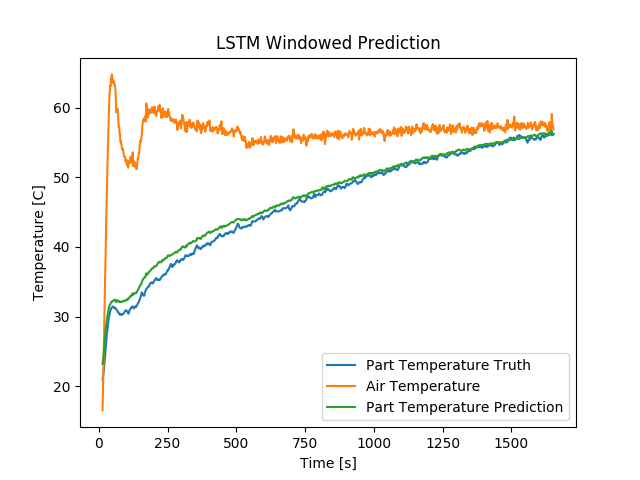
\includegraphics[width=\linewidth]{lstm/lstm_w_predict_april1.png}
    \end{subfigure}
    \begin{subfigure}{.5\linewidth}
    	\centering
    	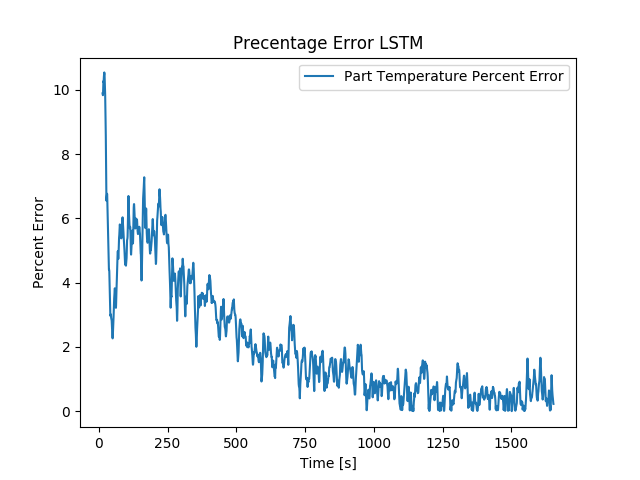
\includegraphics[width=\linewidth]{lstm/lstm_w_predict_april1_error.png}
    \end{subfigure}
    \caption{Real Data Predictions Windowed Data 1}
    \label{fig:real_data_window_lstm1}
\end{figure}
\begin{figure}[ht]
    \begin{subfigure}{.5\linewidth}.
        \centering
    	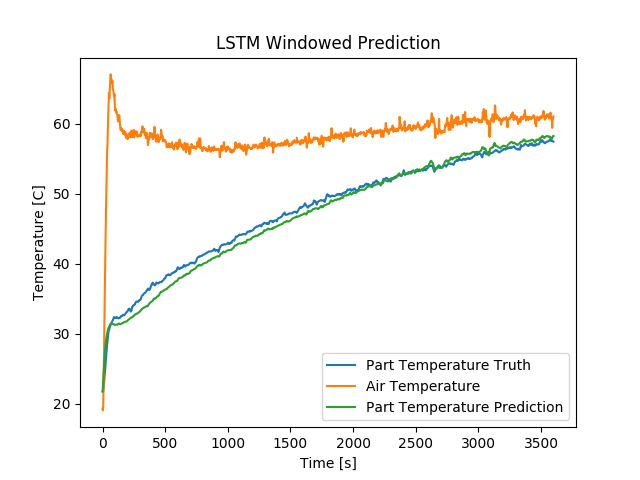
\includegraphics[width=\linewidth]{lstm/lstm_w_predict_april2.png}
    \end{subfigure}
    \begin{subfigure}{.5\linewidth}
    	\centering
    	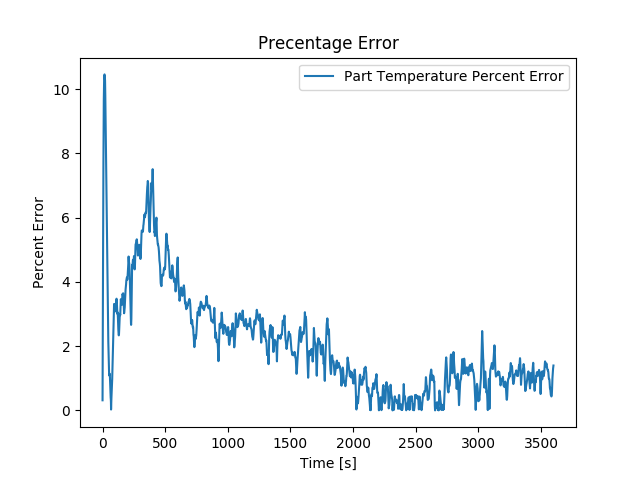
\includegraphics[width=\linewidth]{lstm/lstm_w_predict_april2_error.png}
    \end{subfigure}
    \caption{Real Data Predictions Windowed Data 2}
    \label{fig:real_data_window_lstm2}
\end{figure}
\newpage

\subsection{Soak Time Determination with LSTM}
The LSTM can also be used to make predictions from air data while the run is executing. This means that not all air temperature data is available so it is instead extrapolated to try and evaluate when the run should be finished. The simplest way to predict what the air temperature will do is to extrapolate by assuming it will hold the same temperature now until the end. Alternatives to this method include trying to do a polynomial regression or creating a neural network which predicts on air temperature. The extrapolation happens continually until a consensus on soak time can be made. \\\\
Below in Figure \ref{fig:live_predict} is an example of a prediction being made half way through one of the data sets. Here the soak time is set so that the part temperature should be within 5 percent of 55$^\circ$C so within about 53$^\circ$C and 57$^\circ$C. In Figure \ref{fig:live_predict} the prediction is being made at the blue vertical line using extrapolated data shown in red, the predicted soak time is shown in grey and the true prediction using part temperature truth is shown in black. It can be seen that the part temperature truth lost accuracy due to the extrapolation of air temperature. Click or double click on Figure \ref{fig:live_predict_gif} below to see a video of the live prediction being graphed out a step rate of roughly a prediction every five seconds.
%\href{movie.avi}{\includegraphics{video.avi}}
%\movie[options]{placeholder box}{video.avi}
%\href{movie.avi}{\movie[height = 0.1 \textwidth,width =\linewidth,showcontrols]{}{video.mpg}}
\begin{figure}[ht]
    \begin{subfigure}{.5\linewidth}.
        \centering
    	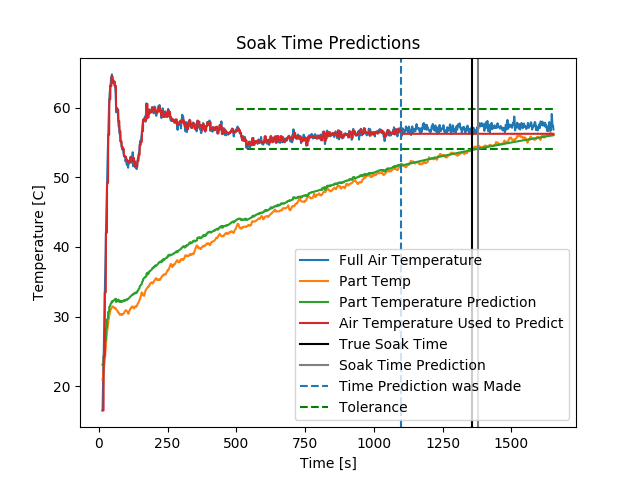
\includegraphics[width=\linewidth]{lstm/0plot_prediction_266.png}
    \end{subfigure}
    \begin{subfigure}{.5\linewidth}
    	\centering
    	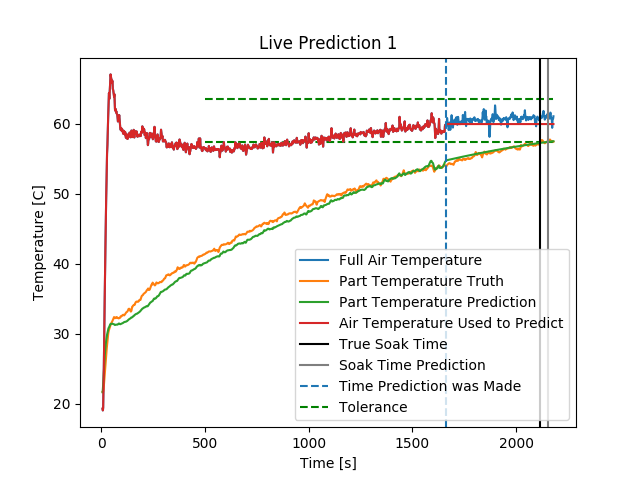
\includegraphics[width=\linewidth]{lstm/1plot_prediction_306.png}
    \end{subfigure}
    \caption{Live Predictions Windowed Data 1 \& 2}
    \label{fig:live_predict}
\end{figure}
\begin{figure}[h]
\centering
\begin{overpic}[width=0.5\textwidth]{lstm/0plot_prediction_266.png}
 \put (0,0){\includemovie[poster,text={\small(Click)}]{.5\textwidth}{6cm}{other/vid.mp4}}
\end{overpic}
\caption{Prediction video showing live prediction (double click, works in firefox), or follow the \href{https://www.youtube.com/watch?v=Oj7pGAFx5Rw&feature=youtu.be}{\textcolor{blue}{\underline{Link}}}}
\label{fig:live_predict_gif}
\end{figure}
\newpage
In Figure \ref{fig:live_predict_36} below, predictions were made on extrapolated data every five seconds. The plot in Figure \ref{fig:live_predict_36}a shows vertical lines in grey for every soak time that was predicted and a single black line for the true soak time. Figure \ref{fig:live_predict_36}b is a plot which shows the predicted soak time versus when that prediction was made. If the prediction is on the left half of the orange line, then that means it is predicting a soak time that is in the future. Once it starts predicting on a soak time in the past, the greatest confidence in accuracy has been achieved. One could then make a control decision to use the prediction that occurs as close as possible to the orange line to obtain the best accuracy. Using this control choice, a result was found where the estimated soak time of 1338.656 seconds versus the real soak time of 1356.877 seconds was found. This would result in a soak time about 20 seconds shorter than needed in a run which takes 22.3 minutes to complete. The other run estimated soak time as 2029.401 seconds when the true soak time was 2115.839 seconds and was 86 seconds off in a run that is 2179.91 seconds or 36.3 minutes long. It can be seen that as the run progresses and gets closer to the true soak time, its accuracy increases and converges to its final prediction. There is a small error in the soak time determined as the prediction is slightly different than the true part temperature curve.
\begin{figure}[ht]
    \begin{subfigure}{.5\linewidth}.
        \centering
    	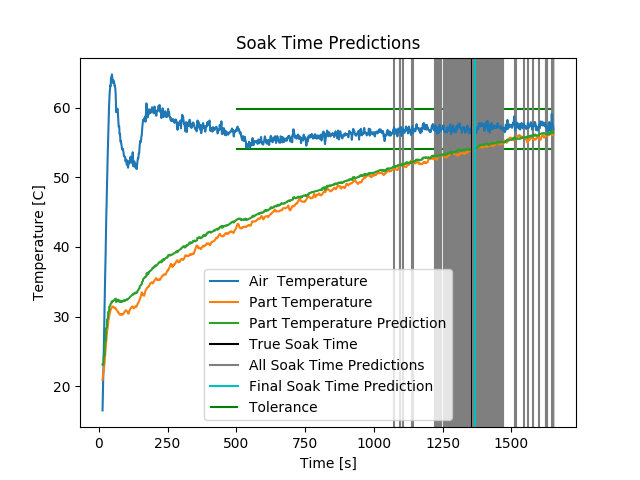
\includegraphics[width=0.9\linewidth]{lstm/soak_time_predictions.png}
        \caption{Soak Time Prediction Made every 5 seconds, Correct Prediction in Black, LSTM Predictions in Cyan/Grey}
    \end{subfigure}
    \begin{subfigure}{.5\linewidth}
    	\centering
    	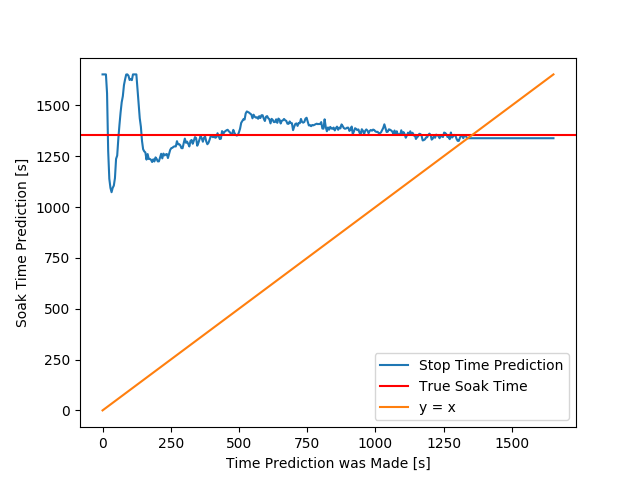
\includegraphics[width=0.9\linewidth]{lstm/soak_time_predictionsb.png}
        \caption{Soak Time Prediction and When it was made}
    \end{subfigure}
    \caption{Live Predictions}
    \label{fig:live_predict_36}
\end{figure}\clearpage
\subsection{Forward Prediction with LSTM}
It is also possible to train on every trial that is available in our data set then extrapolate the trend of air temperature to try to predict the future. This has use cases in seeing where the internal temperature is and how it will be in the future. This shows how soak time can be determined before it is reached allowing a control decision to be made. The simple LSTM’s prediction is shown below in Figure \ref{fig:Future_predct_win}. The trends are sensible except for the 40$^\circ$C run.
\begin{figure}[ht]
    \begin{subfigure}{.33\linewidth}.
        \centering
    	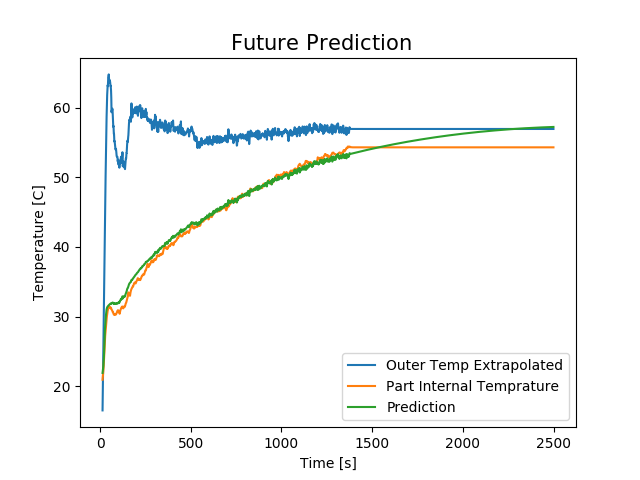
\includegraphics[width=\linewidth]{lstm/predict_f_w2.png}
    \end{subfigure}
    \begin{subfigure}{.34\linewidth}
    	\centering
    	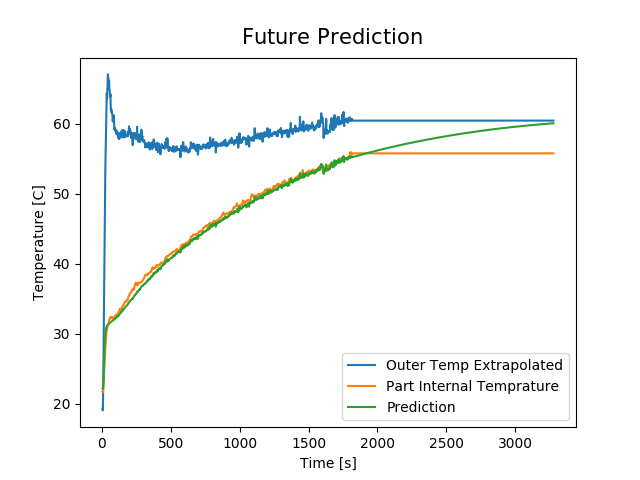
\includegraphics[width=\linewidth]{lstm/future_predict2.png}
    \end{subfigure}
    \begin{subfigure}{.33\linewidth}.
        \centering
    	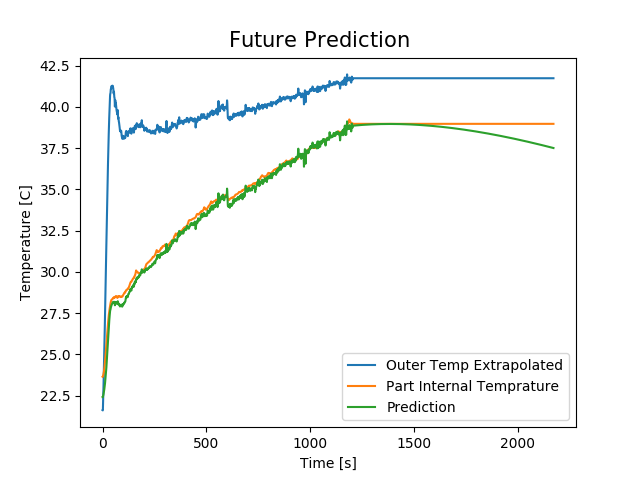
\includegraphics[width=\linewidth]{lstm/future_predict3.png}
    \end{subfigure}
    \caption{Future Data Predictions Simple Method}
    \label{fig:Future_predct_simple}
\end{figure}
\newline
Below in Figure \ref{fig:Future_predct_win} is the LSTM prediction into the future with the LSTM windowed method. As the air and part temperature converge the part temperature's slope does not decrease as expected. This would most likely result in an underestimate in soak time. Future predictions are an interesting look into how the LSTM believes the run will progress. It is hypothesized that with data that fully converges, these predictions would become more accurate. 
\begin{figure}[htb]
    \begin{subfigure}{.33\linewidth}.
        \centering
    	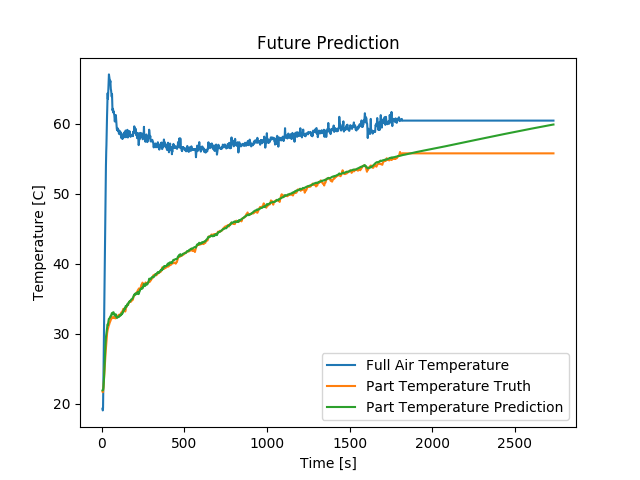
\includegraphics[width=\linewidth]{lstm/lstm_w_future1.png}
    \end{subfigure}
    \begin{subfigure}{.33\linewidth}
    	\centering
    	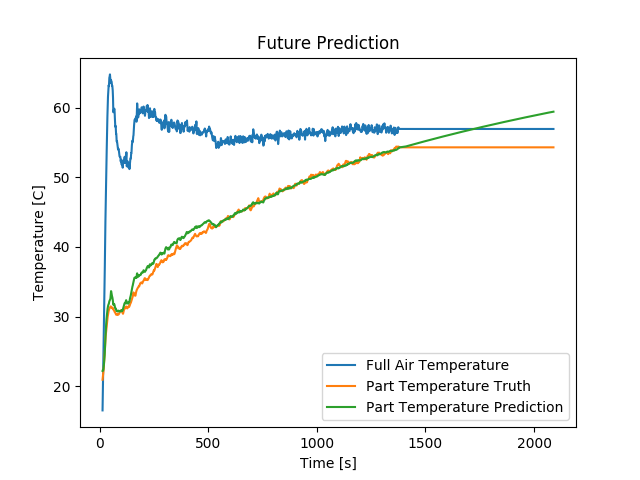
\includegraphics[width=\linewidth]{lstm/lstm_w_future2.png}
    \end{subfigure}
    \begin{subfigure}{.33\linewidth}.
        \centering
    	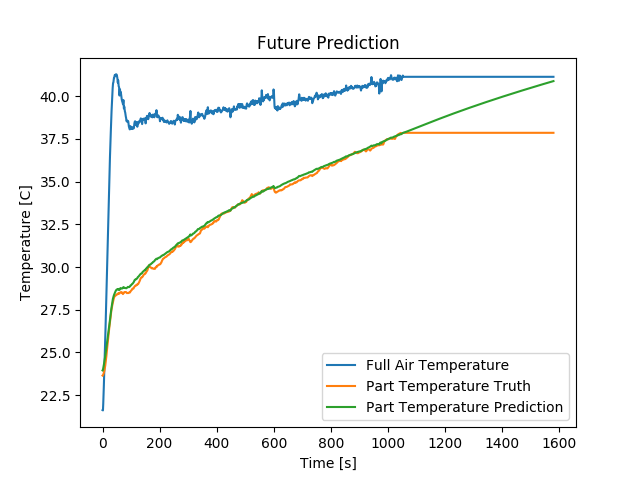
\includegraphics[width=\linewidth]{lstm/lstm_w_future3.png}
    \end{subfigure}
    \caption{Future Data Predictions Using Windowed Method}
    \label{fig:Future_predct_win}
\end{figure}
\clearpage
\subsection{Random Forests}
Random Forests operate on two main principles, decision trees and bagging. While according to \cite{RF}, Random Forests are popular mostly in classification tasks, it is a versatile algorithm that can be used to solve other tasks, such as regression. According to \cite{RF}, "A decision tree is a set of questions organized in a hierarchical manner and represented graphically as a tree". For each input, the decision tree asks successive questions about its known properties and splits into different paths. Depending on the path traversed through the tree, the questions asked will differ. Once the terminal leaf node (end of the path) is reached, the output is predicted.
\begin{figure}[!htb]
    \centering
    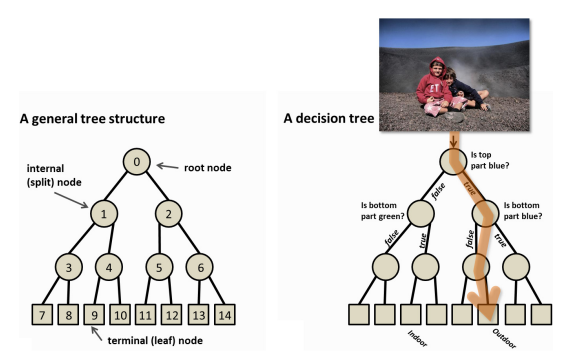
\includegraphics[width=0.5\linewidth]{other/decision_tree_RF.png}
    \caption{Diagram of Decision Tree Structure retrieved from \cite{RF}}
\end{figure}
\\\\To decide how paths are split, split functions based on metrics such as Information Gain, Gini Index, or Mean Squared Error are used. In Scikit-Learn's implementation of decision trees and Random Forests for regression, Mean Square Error is used by default (Eq. \ref{mse}) where $m$ represents a node, $R_{m}$ represents a region, and $N_{m}$ is the number of observations. Mean Absolute Error can also be selected as a split function for regression and is shown in Equation \ref{MAE}.
\begin{equation}
\bar{y}_{m} = \frac{1}{N_{m}}\sum_{i\in N_{m}}y_{i}    
\end{equation}

\begin{equation}
\label{mse}
    H(X_{m}) = \frac{1}{N_{m}} \sum_{i \in N_{m}}(y_{i} - \bar{y}_{m})^2
\end{equation}

\begin{equation}
\label{MAE}
    H(X_{m}) = \frac{1}{N_{m}}\sum_{i \in N_{m}}\mid y_{i} - y_{m}\mid
\end{equation}\\\\
Random Forests use the concept of bagging and an ensemble of decision trees to increase the performance over an individual decision tree. Bagging is a technique in which several weak learners, in this case decision trees, are trained on bootstrapped data sets with randomly selected features. Bootstrapped data sets for each decision tree are created by sampling the training data set with replacement, effectively resulting in different data sets. By randomly training decision trees on bootstrapped data sets, the correlation between each tree is reduced, improving generalization and robustness of the ensemble \cite{RF}.
\subsection{Random Forests Parameters \& Performance}
In this section, we analyze the parameters and performance of the Random Forests machine learning algorithm on the generated and real recorded data. 

\subsubsection{Parameters}
While there are various parameters such as the number of estimators, criterion, maximum depth of the tree, the minimum number of samples required to split a node, and the minimum number of samples required to be a leaf node, the parameters we used in our Random Forest model were left at the default settings. The reasoning behind this decision was because Random Forests are known to typically require minimal parameter tuning. Additionally, we did not have enough real-world data sets to cross-validate and tune the performance of our model before validating on a test set.

\subsubsection{Simulated Data}
Using simulated data, we can test the scenario in which we have a large pool of data and want to make a prediction on unseen data. The performance of Random Forests was evaluated with leave-one-out cross validation. In leave-one-out cross validation, given a pool of data sets, one data set is selected for testing while the remaining data sets are used as a training set. The score for each data set was then averaged which gives us our cross validation score. Scikit-Learn determines the performance of a model using $R^2$ which is determined by Equation \ref{r2} where $u$ is the residual sum of squares, $v$ is the total sum of squares, and $\bar{x}_{y_{true}}$ is the average of the true output labels. The score ranges from a value of 0-1 where 1 is the best possible score.

\begin{equation}
\label{r2}
    R^{2} = (1-\frac{u}{v}) \\
\end{equation}

\begin{equation}
        u = \sum (y_{true} - y_{pred})^{2}
\end{equation}

\begin{equation}
    v = \sum (y_{true} - \bar{x}_{y_{true}})^{2}
\end{equation}

In our testing, Random Forests performed quite well on simulated data and managed to get a cross validation score of 0.9986. Thus we can determine that on simulated data, Random Forests are a suitable method. An example of one of the tests in Figure \ref{RF_sim} shows that the ability of the Random Forest is near perfect. In this case, the percent error of a prediction at any given time constantly remains below 5\% as seen in Figure \ref{RF_sim_err}. The performance of the Random Forest appears to worsen as the slope of the internal temperature curve decreases, however once the internal temperature curve begins to flatten and the soak temperature is met, the Random Forest predictions stabilize.

\begin{figure}[ht]
    \begin{subfigure}{.5\linewidth}.
        \centering
    	\includegraphics[width=\linewidth]{other/RF_prediction_simulated.png}
        \caption{Prediction with Random Forests}
        \label{RF_sim}
    \end{subfigure}
    \begin{subfigure}{.5\linewidth}
    	\centering
    	\includegraphics[width=\linewidth]{other/RF_error_simulated.png}
        \caption{Percent Error}
        \label{RF_sim_err}
    \end{subfigure}
    \caption{Simulated Data Performance using Random Forests}
\end{figure}

\subsubsection{Real Data}
When testing on our real-world data, we once again used leave-one-out testing. In this case since the amount of data we have is minimal, we will look at the results of each test individually. As our data was initially very noisy, we first ran our data through a Kalman filter before training the Random Forest. Looking at the results of max60run1 in Figure \ref{rf601} and \ref{rf601err}, we can see that the Random Forest has decent performance with an $R^2$ score of 0.9608 and typically has a \% error of less than 5\%.

\begin{figure}[ht]
    \begin{subfigure}{.5\linewidth}.
        \centering
    	\includegraphics[width=\linewidth]{other/RF_prediction_real.png}
        \caption{Prediction with Random Forests}
        \label{rf601}
    \end{subfigure}
    \begin{subfigure}{.5\linewidth}
    	\centering
    	\includegraphics[width=\linewidth]{other/RF_error_real.png}
        \caption{Percent Error}
        \label{rf601err}
    \end{subfigure}
    \caption{Real Data Performance using Random Forests - Testing max60run1}
\end{figure}

For max60run2 in Figure \ref{rf602} and \ref{rf602err}, the performance is initially quite good before diverging around the 350 second mark. Around the 700 second mark, the predictions became very unstable before stabilizing when the part gets close to the designated soak temperature. The poor performance in this case can likely be attributed to over-fitting due to a lack of variety in data. 

\begin{figure}[ht]
    \begin{subfigure}{.5\linewidth}.
        \centering
    	\includegraphics[width=\linewidth]{other/RF_prediction_real2.png}
        \caption{Prediction with Random Forests}
        \label{rf602}
    \end{subfigure}
    \begin{subfigure}{.5\linewidth}
    	\centering
    	\includegraphics[width=\linewidth]{other/RF_error_real2.png}
        \caption{Percent Error}
        \label{rf602err}
    \end{subfigure}
    \caption{Real Data Performance using Random Forests - Testing max60run2}
\end{figure}

On the max40 run, in Figure \ref{rf40} and \ref{rf40err}, the performance as expected is incredibly poor. This poor performance is expected as the Random Forest was not trained on a temperature curve with a maximum temperature of 40$^\circ$C. The typical scenario that should be expected is to train the model on a range of temperature curves where the test data set will fall in between.

\begin{figure}[ht]
    \begin{subfigure}{.5\linewidth}.
        \centering
    	\includegraphics[width=\linewidth]{other/RF_prediction_real3.png}
        \caption{Prediction with Random Forests}
        \label{rf40}
    \end{subfigure}
    \begin{subfigure}{.5\linewidth}
    	\centering
    	\includegraphics[width=\linewidth]{other/RF_error_real3.png}
        \caption{Percent Error}
        \label{rf40err}
    \end{subfigure}
    \caption{Real Data Performance using Random Forests - Testing max40}
\end{figure}
\clearpage

\section{Final Design Evaluation} \label{Evaluation}
\subsection{Assessment of Final Design}
Upon evaluation of the project requirements, needs, and constraints identified, it can overall be stated that the design project was a success and completed to the satisfaction of the stakeholders. The primary deliverable of the project was to develop a process for predicting the lag temperature of the metal cylinder using a machine learning algorithm and to use the information to estimate the soak time. We were able to accomplish our objective using Python along with LSTM neural networks and Random Forests for our machine learning algorithms. A comparison of the effectiveness of the LSTM method and Random Forests method can be seen in Figure \ref{fig:real_data_error_rs_lstm1} and Figure \ref{fig:real_data_error_rs_lstm2}. It can be seen from the graphs that the LSTM method is overall more reliable and superior compared to the Random Forests method, as the percent error is generally smaller, more consistent, and less sporadic. The error patterns observed for LSTM represent mostly an offset whereas the patterns observed for Random Forests are more random. Furthermore, the LSTM method is more effective for determining soak time as the prediction by the end of the cycle is more accurate. The estimation of the soak time was implemented into our Python scripts. The system designed for this project establishes an Industry 4.0 framework that can be further expanded upon, and overall the final design is an effective proof of concept for demonstrating the feasibility of this system for composites manufacturing. A practical solution for finding the soak time was implemented in a testing process where it is otherwise unknown.\\\\
In consideration of our other project needs and constraints, we were able to improve and further optimize the data collection process. Better thermistors were purchased and their optimal placement was determined through testing. An ADC was also purchased and these changes allowed us to improve accuracy in our sensor readings and confirm that our results were consistent. The signal-to-noise ratio was taken into consideration as we ran the collected data through filters in order to boost the signal-to-noise ratio. The budget constraint was not a concern, as roughly half of the budget was used throughout the entire project. Safety precautions were always taken while testing in the lab and no danger was ever present. \\\\
One disappointment in our project is that only a small sample of valid data was collected and used for developing the machine learning processes. The small amount of data retrieved was due to limited access to the Composites lab following the COVID-19 outbreak. With minimal data collected, the integration of cloud storage through IBM Cloud was invalidated as it would not be useful for a small data set. Ultimately, most of the requirements, needs, and constraints established by the stakeholders were successfully accommodated and fulfilled. 

\begin{figure}[ht]
    \begin{subfigure}{.5\linewidth}.
        \centering
    	\includegraphics[width=\linewidth]{other/RF_error_real2.png}
    \end{subfigure}
    \begin{subfigure}{.5\linewidth}
    	\centering
    	\includegraphics[width=1.01\linewidth]{lstm/run2_rescale.png}
    	\vspace{.05pt}
    \end{subfigure}
    \caption{Real Data Percent Error Comparison}
    \label{fig:real_data_error_rs_lstm1}
\end{figure}
\begin{figure}[ht]
    \begin{subfigure}{.5\linewidth}.
        \centering
    	\includegraphics[width=\linewidth]{other/RF_error_real.png}
    \end{subfigure}
    \begin{subfigure}{.5\linewidth}
    	\centering
    	\includegraphics[width=1.01\linewidth]{lstm/run1_rescale.png}
    	\vspace{.05pt}
    \end{subfigure}
    \caption{Real Data Percent Error Comparison}
    \label{fig:real_data_error_rs_lstm2}
\end{figure}
\newpage
\subsection{Coronavirus Restrictions}
Due to closure of non-essential laboratories at UBCO in response to COVID-19 as of March 17, 2020, there were a number of topics we were unable cover or implement. In particular, we were unable to gather more reliable data using our redesigned  Raspberry Pi based data acquisition unit. With more data, we would be able to more thoroughly validate our machine learning models. In addition, while the code to predict internal temperature in real-time exists, as we were unable to gain access to the laboratory, we were unable to implement or test this feature with the heat chamber.

\subsection{Recommendations for Future Work}
There are a number of recommendations that can be made for further progressing this project. Some suggestions include: further testing, improving the simulations for generated data, data assimilation, and transfer learning. 
\subsubsection{Further Testing}
One avenue for future work is expanding upon the machine learning process through further testing. This includes gathering additional data for the aluminum cylinder used in this project as well as a comparable volume of data for other parts consisting of different materials and shapes to be used for further training the machine learning models. As it is eventually the goal to implement this type of system for determining the soak time for composite materials, it is necessary to incrementally train and update the machine learning models developed for this project to accommodate other parts and materials before being accessible to composites. \newline
\begin{wrapfigure}{r}{0.5\textwidth}
  \vspace{-50pt}
  \begin{center}
    \includegraphics[width=0.50\textwidth, height = 80mm]{other/filt_data_circle.png}
  \end{center}
  \vspace{-20pt}
  \caption{Filtered Data showing }
  \label{fig:filtered_data_circle}
  \vspace{-20pt}
\end{wrapfigure}
Another test we wanted to perform but were not able to due to separation of the logger and PI controller was to extract the duty cycle of the PI controller over the run. As seen in Figure \ref{fig:filtered_data_circle} to the right and circled in red, there is a steep rising curve initially for the part temperature which is likely due to an increased amount of heat transferred through radiation because the infrared lamp was on for high duty cycles in our collected data, and without extracting the duty cycle we could not use that information at the initial point in time. It is expected that with this additional information the machine learning algorithm would have an easier time adjusting for the offset that the part temperature is at throughout the run.  \\

\subsubsection{Improving Simulations}
There are some limitations in the simulations performed for this project, and further improvements in the simulation parameters would aid in validation of the machine learning models and the data collected. In the MATLAB simulations performed, a two-dimensional rectangle was modeled to approximate the three-dimensional cylinder used in the project. While this was a simpler process, more accurate and reliable data could be generated by importing an identical 3D mesh of the cylinder for the simulation runs.  \\\\
Another adjustment that could be made to the simulations is to account for more parameters. For simplicity, the model used for the simulations referenced in this report only account for conductive heat transfer, but a more thorough model would also account for convective heat transfer and radiation. The thorough model is more useful as it provides a more accurate and practical view of the heating system and its properties.
\subsubsection{Data Assimilation}
Another possible improvement for this project is data assimilation which is the use of computer generated data such as a simulation combined with real world data to create synthetic data which is assimilated with the real data to train a neural network. As we have both of these components, further testing could be implemented. It was found that the simulation needed to be tweaked further to attain data that improved the prediction ability. A small amount of testing was conducted in this area on the LSTM model but it was found that it did not improve the prediction ability on real data. It may have only decreased over-fitting of the model. It is challenging to come to a definite conclusion, especially since the simulated data vastly outnumbers the real data. The most interesting result from data assimilation would be to decrease the number of real runs that need to be conducted therefore this would be an area for further research.
\subsubsection{Transfer Learning}
Lastly, a worthwhile concept to look into is Transfer Learning. Transfer Learning is a domain of machine learning which uses the training data or model from one problem and adapts it towards a new but related problem. As we saw some cases of over-fitting during our testing, transfer learning could possibly used as an option to counteract over-fitting and improve generalization performance. In particular, Transfer Learning could work well in cases where we have a limited amount of training data for a certain target scenario (e.g. new material, different object geometry) but have related data from previous experiments or other data sets. Some interesting Transfer Learning methods to look into include \cite{daume07easyadapt}, and \cite{DBLP:journals/corr/SunFS15}. Both of these Transfer Learning methods have good performance and are simple to implement and require less than 10 lines of code. 
\clearpage

\section{Conclusion}
Through this Capstone project, we were able to collaborate with the UBC Okanagan Composites and Optimization laboratory to create an Industry 4.0 solution to the composites manufacturing process in the lab. The objective was to develop a proof of concept machine learning process to optimize the curing cycle of composite materials by estimating the soak time. To develop our framework, an aluminum cylinder was used for testing and gathering data for the machine learning algorithm. Through our project, we were able to improve the data acquisition process by incorporating a Raspberry Pi and ADC to the test configuration. These devices were used to make the curing process simpler and to retrieve more accurate readings from the temperature sensors. From the literature review and research performed, we decided on using Random Forests and LSTM for our machine learning process in order to compare the results given by different methods and to observe which is more effective for our needs. Python was decided for implementing the machine learning algorithms for its extensive selection of machine learning libraries and its accessibility. \\\\
An engineering approach was adopted to resolve concerns that arose during the development of this project. To address the concern of noise, we experimented with different filters and analyzed their effectiveness to improve the signal-to-noise ratio while remaining accurate and seeing how it affected the results of the machine learning processes. Ultimately, we found that noise had little effect on the machine learning algorithms or on the soak time of a test run. Simulations were also performed in MATLAB to complement the real data that was obtained. The simulations allowed us to further understand the test process and allowed us to generate a greater data set to help the modeling of the machine learning algorithms. We developed two machine learning algorithms one using Random Forests and another using a LSTM model. After extensive development on the machine learning processes, we were able to generate predictions with a percent error under 4\% for an entire run. The machine learning algorithms were then applied to predict the soak time of a simple metal part. This could then be used to make a control decision when to stop a curing cycle. The machine leaning algorithm was also used to try and predict how the part would heat up in the future. Despite limitations raised due to the COVID-19 outbreak, we were ultimately able to successfully fulfill the stakeholder's needs. For further development on this design, our recommendations include: accumulation of more data for further fine-tuning of the machine learning processes, more advanced simulations, data assimilation, and transfer learning. 
\clearpage

\addcontentsline{toc}{section}{Appendix} \label{Appendix}
\section*{Appendix}
\addcontentsline{toc}{subsection}{Github}
\subsection*{Github}
Link to GitHub: \href{https://github.com/darryllam/CRN_Heat_Chamber}{\textcolor{blue}{\underline{https://github.com/darryllam/CRN\_Heat\_Chamber}}}
\addcontentsline{toc}{subsection}{LSTM Code Usage and weights}
\subsection*{LSTM Model and Weights}
LSTM weights are saved in the git repo to see which weights are used where check the file  \\ CRN\_Heat\_Chamber/python\_src/README which calls the python script to access the weight file.
\begin{itemize}
    \item \lstinline{model_weights_Jup_alt_scale_april.h5}, trained on variable size data found in jupyter folder
    \item \lstinline{model_weights_real_data_1_20_70_april11.h5}, trained on kalman data kalma\_max40.csv \& kalma\_max60run2.csv 
    \item \lstinline{model_weights_real_data_40_20_70_april11.h5}, trained on kalman data kalma\_max2.csv \& kalma\_max60run1.csv 
     \item \lstinline{model_weights_real_data_2_20_70_april11.h5}, trained on kalman data kalma\_max40.csv \& kalma\_max60run1.csv
     \item \lstinline{model_weights_train_all.h5}, trained on kalman data kalma\_max40.csv \& kalma\_max60run2.csv\\ \& kalma\_max60run1.csv
    \item \lstinline{model_weights_train_all_w.h5}, trained on kalman data kalma\_max40.csv \& kalma\_max60run2.csv \& kalma\_max60run1.csv with window size 50
    \item \lstinline{model_weights_real_window1.h5}, trained on kalman data kalma\_max40.csv \& kalma\_max60run2.csv with window size 50
    \item \lstinline{model_weights_real_window2.h5}, trained on kalman data kalma\_max40.csv \& kalma\_max60run1.csv with window size 50
\end{itemize}
\subsection*{LSTM Code Usage}
The code runs in the command line and options are given through command line options. The test path and validation path point to folders only containing csv files. Input file is to input a network model. Out file is the output file to save a network model. The window size, epochs, minimum air temp, maximum air temp can all be adjusted with integers. Values are input to point to columns in the data. See CRN\_Heat\_Chamber/python\_src/README for files which can be used to easily execute the python lstm files using the linux command \lstinline{>>source FILE}. Below is an example.\\
\ttfamily
%\setlength{\parindent}{1}

python3 -i lstmMethod.py -tp ../real\_data\_kalman/train/ -vp ../real\_data\_kalman/test/ \\ -o weights\_real\_test.h5 -w 1 -vcol 2 -stcol 0 -tmcol 1 -min\_temp 15 -max\_temp 70 -e 1 -state 0\\
\rmfamily

-tp is train path
-vp is val/test path
-o is output file for model
or
-i is input weight for model

-w is how many windows you want

-vcol is column of data that holds part temp info
-stcol is column of data that holds time or other data that you want to scale on a per trial basis
-tmcol is air temp column
-min\_temp is minimum temp used when scaling temperature data
-max\_temp is maximum temp used when scaling temperature data

-e is number of epochs to train that data for
-state 0 is to set stateful to be off which is typical
Example for predicting data for future prediction and real time prediction: 
\ttfamily

python3 -i predict\_windows.py -vp ../real\_data\_kalman/test/ -i weights\_real\_test.h5 -w 1 -vcol 2 -stcol 0 -tmcol 1 -min\_temp 15 -max\_temp 70 -future 1.25 -live 900
\rmfamily

-vp is val/test path

-i is input weight for model

-w is how many windows you want

-vcol is column of data that holds part temp info
-stcol is column of data that holds time or other data that you want to scale on a per trial basis
-tmcol is air temp column
-min\_temp is minimum temp used when scaling temperature data
-max\_temp is maximum temp used when scaling temperature data

-future is a fraction which is multiplied by data len to create a longer array, and will be predicting if longer than data\_len. Must be a multiple of batch size 
-live is step size to be making predictions

\addcontentsline{toc}{section}{References} \label{References}
\printbibliography
\end{document}